
\documentclass[runningheads,a4paper]{llncs}
\pagestyle{plain}
\usepackage{amssymb}
\setcounter{tocdepth}{3}
\usepackage{graphicx}

\usepackage{url}
\urldef{\mailsa}\path|{fwei, yupingli}@mail.usf.edu|
\urldef{\mailsb}\path|sanroy@bgsu.edu, xou@usf.edu, woodzltc@gmail.com|
\newcommand{\keywords}[1]{\par\addvspace\baselineskip
\noindent\keywordname\enspace\ignorespaces#1}

% correct bad hyphenation here
\hyphenation{op-tical net-works semi-conduc-tor}

\usepackage{verbatim}
\usepackage{xspace}
\usepackage{float}
\usepackage{graphicx}
\usepackage[font=small,labelfont=bf]{caption}
\usepackage{subcaption}
\def\UrlBreaks{\do\/\do\_\do-}
\usepackage{breakurl}
\usepackage[breaklinks]{hyperref}
\usepackage{tabu}
\usepackage{color}
\usepackage{mathtools}
\usepackage{algorithm}
\usepackage{algpseudocode}
\usepackage{comment}
\usepackage{subscript}
\usepackage[version=3]{mhchem}
\usepackage{setspace}
\usepackage{multirow}
\usepackage{rotating}
\let\labelindent\relax
\usepackage{enumitem}
\usepackage{syntax}
\usepackage{tikz}
\usepackage{amssymb}
\usepackage[strings]{underscore}
\usepackage{array}
\newcolumntype{?}{!{\vrule width 1pt}}
\usepackage{makecell}
%\def\checkmark{\tikz\fill[scale=0.4](0,.35) -- (.25,0) -- (1,.7) -- (.25,.15) -- cycle;} 

\DeclarePairedDelimiter\ceil{\lceil}{\rceil}
\DeclarePairedDelimiter\floor{\lfloor}{\rfloor}
\hyphenation{multi-layered}
\hyphenation{multi-layer}

\newcommand{\etc}{{\it etc}.\xspace}
\newcommand{\etal}{{\it et al}.}
\newcommand{\ie}{{\it i.e.},\ }
\newcommand{\eg}{{\it e.g.},\ }
\newcommand{\aka}{{\it a.k.a.}\ }

\newcommand{\genome}{{Android Malware Genome}\xspace}
\newcommand{\amd}{{Android malware website}\xspace}
\newcommand{\fsize}{{71}\ }
\newcommand{\versize}{{135}\ }
\newcommand{\samsize}{{24,650}\ }

\newif\ifsubmit\submitfalse

\ifsubmit
\newcommand{\xo}[1]{}
\newcommand{\morecite}{}
\else
\newcommand{\xo}[1]{{\color{red}{XO: {#1}}}}
\newcommand{\morecite}{{\color{red}{[citation]}}}
\fi


% \newcommand{\mycomment}[1]{{(\color{red} \bf** #1 **)}}
% \newcommand{\morecite}{\textbf{[citation]}}
\newcommand{\fn}[1]{\textbf{\textit{#1}}}
\newcommand{\pubsite}{\url{http://amd.arguslab.org/}\xspace}
\newcommand{\ptitle}[1]{\vspace{0.2cm}\textbf{#1:}\par}

\newenvironment{smallitem}{\setlength{\topsep}{0.0 truein}
   \begin{itemize}
   \setlength{\leftmargin}{.1 truein}
   \setlength{\parsep}{0.0 truein}
   \setlength{\parskip}{0.0 truein}
   \setlength{\itemsep}{0.0 truein}}{\end{itemize}}

\newenvironment{smallenum}{\setlength{\topsep}{0.0 truein}
   \begin{enumerate}
   \setlength{\leftmargin}{.1 truein}
   \setlength{\parsep}{0.0 truein}
   \setlength{\parskip}{0.0 truein}
   \setlength{\itemsep}{0.0 truein}}{\end{enumerate}}


%\newcommand{\Thetitle}{}
%\newcommand{\Thesubtitle}{[Research Paper]}

\newtheorem{mydef}{Definition}

%\usepackage{etoolbox}
%\makeatletter
%\patchcmd{\maketitle}{\@copyrightspace}{}{}{}
%\makeatother

\begin{document}
%
% paper title
% can use linebreaks \\ within to get better formatting as desired
% \title{A Comprehensive Study of the Current Android Malware Landscape}
\title{Deep Ground Truth Analysis of Current Android Malware}
\author{Fengguo Wei$^1$\and Yuping Li$^1$\and Sankardas Roy$^2$\and Xinming Ou$^1$\and Wu Zhou$^3$}
\institute{$^1$University of South Florida,
$^2$Bowling Green State University,
$^3$Didi Labs.}

% make the title area
\maketitle



\begin{abstract}
\vspace{.02 in}
% The Android platform has captured the majority of the smartphone market share. 
% Unfortunately, 
%The phenomenal success of the Android platform attracted large amount of malware.
To build effective malware analysis techniques and to evaluate new detection tools, 
up-to-date datasets reflecting the current Android malware landscape 
are essential. For such datasets to be maximally useful,
they need to contain reliable and complete information on malware's behaviors and
techniques used in the malicious activities. Such a dataset shall also provide a
comprehensive coverage of a large number of types of malware. 
The \genome created circa 2011 has been the only well-labeled and widely studied dataset the
research community had easy access to\footnote{As of 12/21/2015 the 
Genome authors have stopped supporting the dataset sharing due to resource limitation.}.
But not only is it outdated and no longer represents the current Android malware 
landscape, 
it also does not provide as detailed information on malware's behaviors 
as needed for research.
Thus it is urgent to create a high-quality dataset for Android malware. %  to facilitate
% research in this important area.
% The main challenge 
% is to provide accurate and reliable information for the malware behaviors and
% to scale the analysis at the same time.
While existing information sources such as VirusTotal are useful, 
to obtain the accurate and detailed information 
for malware behaviors, deep manual analysis is indispensable. 
In this work we present our approach to preparing a large Android malware dataset
for the research community. We leverage existing anti-virus scan results
and automation techniques in categorizing our large dataset (containing \samsize malware app samples) 
into \versize varieties (based on malware behavioral semantics) which belong to \fsize malware families.
For each variety, we select three samples as representatives, for a total of 405 malware samples,
to conduct in-depth manual analysis.
% leading to the manual analysis of about 400 malware apps that are representatives of the above varieties, and 
% leverage existing tools to manually analyze 
% these representative apps.
Based on the manual analysis result we generate detailed descriptions of each malware variety's behaviors and include them in our dataset. %  using 
% state-of-the art static analysis tools.
We also report our observations on the current landscape of Android malware as depicted in the dataset.
% We produce detailed documentation of both the manual analysis process and
% the results, and 
%Not only do we provide the research community with the new up-to-date dataset, 
Furthermore, we present detailed documentation of the process used in creating the dataset, including
the guidelines for the manual analysis. 
% the results, and
%Our work is the first that presents a systematic process of analyzing 
%a large number of Android malware samples so that this process can be replicated by other researchers 
%on other Android malware samples in their possession.
We make our Android malware dataset available to the research community. 
%The detailed profile and behavior information about each malware variety can be found at the website \url{http://www.androidmalwaredataset.org/}.
%The complete dataset will be shared upon request with a research purpose.

% Traditional techniques such as clustering 
% analysis cannot be directly applied due to the widespread use of shared third-party 
% libraries and repackaging techniques in the Android malware world. In this work, 
% we leverage antivirus scanning results from VirusTotal and threat reports
% from anti-virus community
% to get family names 
% for the collected Android malware samples. We then refine the malware families through a 
% payload-sharing-based clustering analysis augmented with manual verification, 
% and 
%We perform a comprehensive study of behaviors, techniques, and trend of Android malwares,
%and produce a large labeled dataset with \samsize samples of \fsize malware families
%ranging from 2010 to 2016.
%We further perform automated clustering analysis 
%(augmented with occasional manual study) to categorize
%malware samples in several families while one family may have 30 versions.
%Through manual study of representative samples from each version of each family, we
%produce detailed documentation and list our observations to provide research community with a
%landscape of recent Android malware.
%For each malware family, we study its
%(1) versions with timeline
%and geography;
%(2) installation \& activation strategies;
%(3) behaviors \eg privilege escalation, remote control, financial charges,
%personal information stealing, download \& install application, stealthiness;
%(4) anti-analysis \& obfuscation techniques.
% This dataset will help the Android research community to have an up-to-date 
% understanding of the Android malware landscape and produce better anti-virus 
% solutions in the future. We also present the key observations we made for the
% current Android malware landscape.
\end{abstract}
\vspace{-.03 in}

%%% Local Variables: 
%%% mode: latex
%%% TeX-master: "paper"
%%% End: 

\vspace{-.1in}
\section{Introduction}
\label{sec:introduction}
\vspace{-.02in}

The Android platform continues to dominate the smartphone market
with more than 80\% share according to the study by 
International Data Corporation~\cite{idc} and Gartner~\cite{gartner}.
Over the last five years, the Android world has been changing dramatically with
more features added, and more sensitive operations (\eg banking and wallet) 
becoming popular on smartphones.
Along with the Android platform's popularity, the Android malware has been growing as well,
with more complex logic and anti-analysis techniques. 
%(such as, dynamic loading\morecite, code obfuscation\morecite).

As expected, research groups across academia and industry put
enormous effort to design novel methods to detect Android malware. 
However, the above effort is adversely affected by the lack of clear understanding of 
the latest Android malware landscape. 
A reliable ground truth dataset is essential for building effective 
malware analysis techniques and verifying the validity of new detection methods.
% In order to design effective detection solutions for new Android malware,
% it is necessary to obtain key insights by studying the recent malware behaviors. 
For understanding the nefarious techniques used in the state-of-the-art malware apps, 
{\bf detailed behavior profiles for each malware variety must be provided
in such a dataset}.
While creating such a dataset is a must-do ground work,
this task is extremely difficult.
In particular,
% Unfortunately, such a dataset is extremely difficulty to construct.
%There are significant challenges in creating a new, more up-to-date dataset for Android malware.
%in studying the overall landscape of recent Android malware.
{\bf to provide the rich information for malware behaviors, manual analysis is indispensable.}
However it is not feasible to manually analyze all Android malware at our hands (we have \samsize
from various sources). Thus the first step is to categorize the samples into
semantically equivalent groups; then we only need to study a few samples
from each group.


One can use AV scanning service like
VirusTotal~\cite{virustotal} to group malware samples into families;
however, the family labels returned are often
inconsistent~\cite{hurier2016lack,sebastian2016avclass}.
% The first challenge is due to scalability issue.
Moreover, we observe that malware samples within one family
may actually contain different varieties with different behaviors.
Thus we cannot simply rely upon the grouping provided by AV products, even after being refined
by tools like AVclass~\cite{sebastian2016avclass}.
% It is infeasible to manually study every sample for
% a large family, \eg when the family size is larger than a few hundred.
% The second challenge is due to difficulty in automating the Android malware categorization task.
% We can use clustering to group malware based on their semantic features.
% Unfortunately, traditional PC malware clustering techniques are not readily
% applicable to Android apps due to their excessive usage of 
% shared libraries and the repackaging techniques.
Even if grouping has been done perfectly, the amount of work of manually analyzing
representative apps from each malware variety is still daunting.
Advanced obfuscation methods are
widely adopted in recent Android malware apps, further complicating the manual
analysis process.



%Nevertheless, 
%the Android research community \morecite is still using the dataset from 

Due to the above reasons, there has not been any effort on creating such a
rich Android malware dataset, except for the 
\genome~\cite{zhou2012dissecting} project.
The \genome dataset is no longer
available to researchers due to resource limitations.
 % (which includes analysis of each family)
 % that the community can use.
It provided a malware dataset containing
1260 malware samples categorized in 49 families,
discovered in 2010 and 2011.
%We experimented with this dataset and observed that
We have collected a more recent Android malware dataset from several 
sources (VirusShare, Google Play and third party security companies).
% while the majority
The malware in this collection were discovered between 2010 and 2016. 
We made comparative study of the Genome dataset with our malware samples of 2011 and later,
and found that the majority of the threats in those newer samples are not captured by the 
Genome samples. As a result, we not only need a more up-to-date malware dataset for Android,
we also need one with much richer semantic information than what the Genome dataset provided.



%\genome data is too outdated to capture some of the new threats.
%The \genome  is old, without up-to-date understanding of Android malware,
%and new data set, practical methods cannot designed to capture the new threats.

%Note that there are significant challenges in studying the overall landscape of recent Android malware and their categorization. 
%One challenge is due to scalability issue while another challenge stems from the fact that traditional technique to handle 
%desktop malware does not readily work for the Android domain for the following reasons:
%In particular, security companies receive hundreds of ``potentially malicious'' Android samples everyday \morecite while 
%traditional desktop malware triage process such as malware clustering is not directly applicable to Android domain for following reasons:
%The excessive usage of libraries in the Android world and the repackaging techniques
%adopted by Android malware authors make clustering process challenging - for instance, two malicious Android app samples sharing 
%high level of overall similarity does not guarantee that they belong to the same family.
%And even among the app samples which are labeled with the same family name by anti-virus companies (\eg listed on Virustotal), 
%there may exist significant varieties (sub-families) of different version of malicious payloads.
%On one hand, malware samples with new version payload may break existing malware detection technique, so it is necessary to analyze each version of malicious samples individually.
%On the other hand, it becomes almost infeasible to manually study every sample for a large family; for instance, when a family size is as large as 8000.


\vspace{.1in}

%Understanding of the those techniques will help to (why/what/how)
\noindent {\bf The main contributions of this work are as follows.}
\begin{enumerate}[label=\textbf{\arabic*}.]
\vspace{-.1in}
\item
We present a systematic method of analyzing large volumes of Android malware samples with high
%confidence, which helps us to prepare a large ground truth Android malware dataset.
%This method addressed the scalability challenge by leveraging a two layer grouping technique,
%(1) Group malware samples with same family name, 
%(2) Refine each family to semantically different varieties using clustering analysis.
%We then perform manual analysis on each variety of each family to generate behavior report.
%The final dataset contains \samsize labeled Android malware samples that are classified in \versize varieties within \fsize families, 
confidence, which helps us prepare a large ground truth Android malware dataset with rich profile information.
This method addresses the scalability challenge by leveraging a two-step grouping technique
followed by a systematic and deep manual analysis.
\item We present a detailed guideline for performing the manual analysis so other researchers can 
replicate the process on other Android malware samples in their
possession.
Our manual analysis provides profiles for each variety of the Android malware
regarding their behaviors.
% , we further conduct 
% a comprehensive study to profile
% their behaviors, and monetization methods.
This provides insights into the landscape of the current Android malware.
\item We prepare a comprehensive dataset which contains \samsize labeled Android malware samples that are classified in \versize 
varieties within \fsize families, 
whose discovery dates range from 2010 to 2016. 
%We collected the samples from various sources, including VirusShare, Google Play, and third party security companies.
We publish detailed reports including behavior information for each malware variety at our
\amd \pubsite.
We are sharing the whole dataset with the research community.
%\item We propose a  
%payload sharing based malware clustering approach to
%separate malware samples from a particular family to different versions.
%For each particular version samples, we randomly select xxx samples 
%to conduct detailed manual analysis and verify the correctness of
%clustering results. 
%For each malware family we using cluster analysis to get the different version,
%and for each version of each malware family we detailed analyze the behavior
%it has and write down the document.
% \vspace{-.02in}
% \item 



% In our dataset, we find that 
% (a) since 2012 the percentage of malware varieties that are standalone is increasing and 
% that of repackaged malware is decreasing.
% % 63\%/35\%\footnote{\% of varieties/\% of apps} are standalone apps as opposed to 30\%/7\% being repackaged 
% % apps\footnote{The remaining are cases where an app developer used a malicious library without knowing it.},
% This indicates that malware writers are recently investing more resource in Android malware development;
% (b) the percentage of malware varieties that gain root privilege is decreasing;
% % Only 24\%/5\% malware families attempt to gain root privilege, which shows
% this indicates that Android OS is becoming harder to exploit;
% however, the recent rooting malware are becoming more sophisticated, 
% which can potentially
% make them as complex as PC malware in the near future;
% (c) more Android malware % 63\%/79\%
% apply anti-analysis techniques to evade detection, which
% indicates the urgent need of advanced de-obfuscation and 
% dynamic analysis tools;
% % within one malware family as well as between different malware families.
% (d) We observe that
% malware are evolving towards monetization.
% % 61\%/86\% adopt at least one monetization method;
% % among them, 52\%/85\% are related to banking, ransom and aggressive advertisement, 
% 61\% of malware varieties adopt at least one monetization method;
% among them, 52\% are related to banking, ransom and aggressive advertisement, 
% which is different from old methods such as subscribing to premium services.
% %this shows that the current malware apps use a diversity of ways to get more revenue.
% %Futhermore, other growing techniques support the goal of generating more revenue.
% %For instance, applying device-admin privilege helps malware gain more control of infected device.
% %The more efficient persistence techniques keep malware operating longer, and
% %the extensive use of anti-analysis techniques makes the malware harder to be detected and removed.
% %(1) Obtaining system-admin privilege has become more popular,
% %because it can give the malware the power to encrypt the file system,
% %modify PIN code, wipe user data; and make it difficult to be uninstalled;
% %(2) Using timer or {\em AlarmManager} to schedule
% %timing task periodically (\eg collecting victim's data and fetching command from the C\&C
% %server) has become more dominant in recent malware design;
% %an extreme use of this is found in recent ransomware apps;
% %(3) Malware design is moving towards using persistence techniques, \eg 
% %evidence-cleaning, prevention-from-destruction methods are invented to keep the malware
% %staying longer on the infected device.
\end{enumerate} 


% \vspace{-.05in}
The rest of the paper is organized as follows. Section~\ref{sec:data} discusses
the process of preparing the dataset.
Section~\ref{sec:profile} discusses in details the behaviors and techniques of malware in our dataset,
and Section~\ref{sec:evolution} discusses our analysis and observation of the malware evolution trends.
%We summarize the main findings of our analysis in Section~\ref{sec:value},
We discuss related research in Section~\ref{sec:related},
and conclude in Section~\ref{sec:conclusion}.

%%% Local Variables: 
%%% mode: latex
%%% TeX-master: "paper"
%%% End: 

\section{Methodology}
\label{sec:data}

\vspace{-.3in}
\begin{figure}[h]
\centering
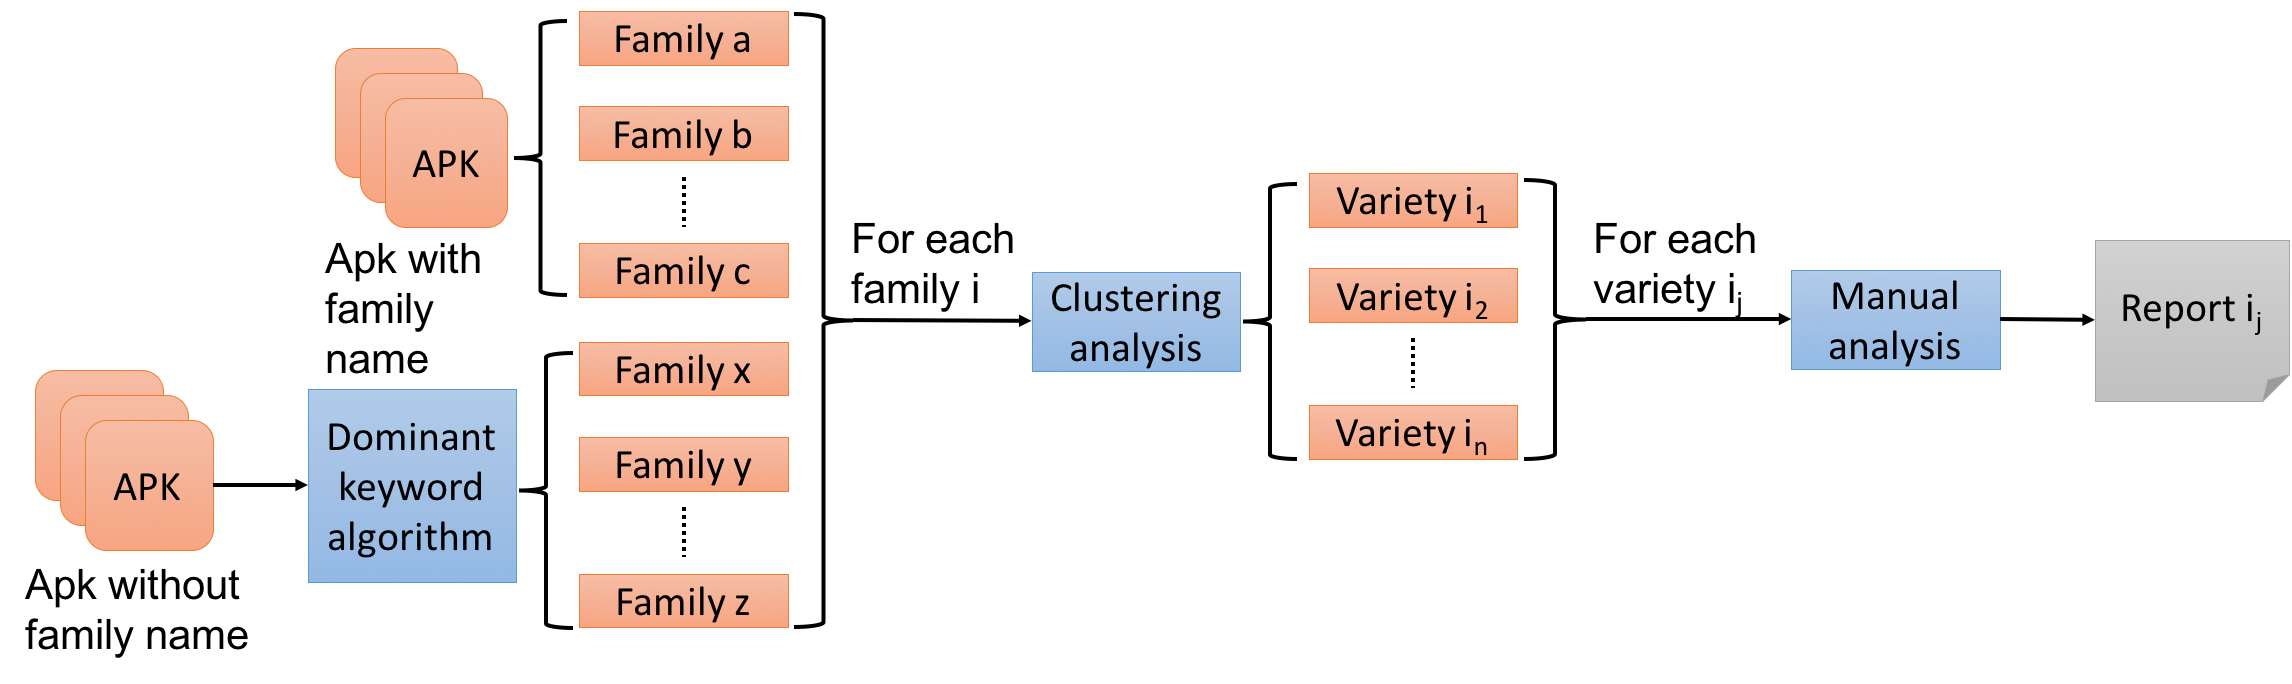
\includegraphics[width=4.5in]{fig/method-pipe.png}
\caption{Methodology pipeline: 
After malware families are identified, each family is categorized into semantically different varieties.
For each variety we generate a malware behavior report,
which is available at our \amd.}
\label{fig:methodpipe}
\end{figure}

We collect Android malware apps from multiple sources, analyze the samples, and report their detailed
behaviors.
Figure~\ref{fig:methodpipe} illustrates the pipeline of the methodology, which consists of
a two-step grouping process
followed by a manual procedure:
(a) Group malware samples with the same family name, 
(b) Categorize each family into semantically different varieties using a customized clustering analysis,
(c) Conduct a systematic and deep manual analysis for each variety of malware samples to obtain the accurate
    and detailed behavior information for the malware.

\subsection{Identifying Malware Families}
\label{sec:data:family}
%We collected the malware samples from various sources, including VirusShare, Google Play, and third party security companies.
%These malware apps were discovered (\ie they appeared in public) between 2010 and 2016. 

After raw malware samples are collected, it is an industry common practice to assign a family name
to each app and group malware into families. The family name typically indicates the origin of the 
malware samples, such as in terms of the malware writer, malicious campaign, individual characteristics, \etc


We collect sample apps from multiple sources, including
VirusShare, Google Play\footnote{Some malware can get pass Google's vetting system and end up in Google Play.},
and third party security companies.
%Most of the sources (in particular, VirusShare and Google Play) 
%do not provide the apps with an assigned family name. 
Most of the malware do not have an assigned malware family name.
For such ``unassigned'' apps, the first step is to identify the family name.

\subsubsection{Challenge}

Existing state-of-the-art malware scanning service such as VirusTotal often
provides multiple labels when it lists the scan result for an app using
different anti-virus tools. However, due to inconsistent naming schemes from different
anti-virus vendors~\cite{maggi2011finding,mohaisen2014av},
how to reliably identify a family name for a malware sample is a challenge.

%Android malware dataset (\amd) contains malware apps 
%we collected from various sources, including VirusShare,
%Google Play, and third party security companies.
%Those malware apps were discovered between 2010 and 2016.

%The apps that we got from third party security companies 
%came with the malware family names, and for each family we received 
%a high-level report.
%App samples from other sources (\eg VirusShare, Google Play) are not labeled with malware family
%name, or some of them may not even are malware.

\subsubsection{Solution}

We collected 1,464,590 unassigned app samples,
and applied the following two steps:

\begin{enumerate}[label=\alph*)]
%So, to know whether an app is malware and if yes, then to identify its family name we use the following method.
\item For each app $x$ we get scan results of 55 antivirus products from VirusTotal (each result is either a candidate label or not-a-malware).
If at least 50\% of anti-virus products used in the VirusTotal recognize app $x$ as a malware, 
we mark $x$ as malware and move to the second step to obtain the family name.
After this step, out of the collected apps, 1,216,885 are not labeled as malware by any AV
product; about 195,185 are labeled as malware by some AV but did not reach the 50\% threshold.
We have 52,520 apps left.
\item We obtain the family name of app $x$ using a ``dominant keyword algorithm''
as follows.
First, take the scanning results of app $x$ from VirusTotal as label candidates.
Second, normalize all the label candidates into individual English keywords,
and meanwhile remove generic English keywords if any, \eg Trojan, Android, A, B,~\etc
There are a few hundred English keywords extracted and we identify the generic terms manually.
Finally, we use the \emph{dominant keyword} among the remaining labels as the family name.
A keyword is dominant when: 
(a) the count of the keyword is greater than 50\% of the anti-virus products used in the VirusTotal result; 
(b) the count of the most popular keyword is equal or more than twice of any other keyword, 
\ie there are no ambiguous labels that are highly popular at the same time.
If for an app no dominant family name is found, we filter out the app from our dataset.
\end{enumerate}


\begin{figure}[t]
\centering
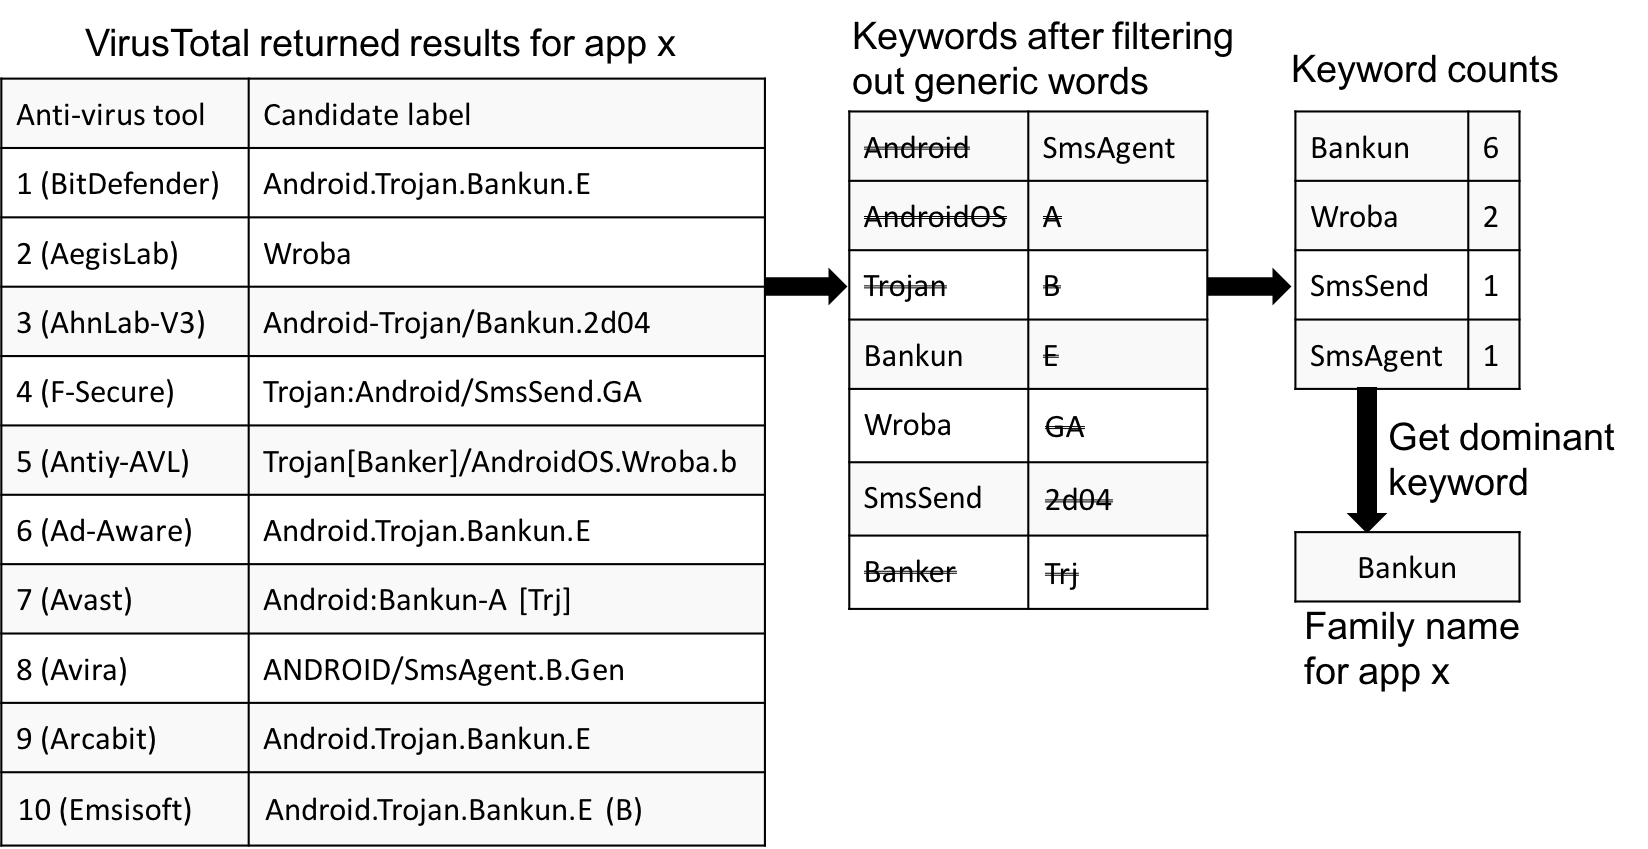
\includegraphics[width=3.8in]{fig/dominant.png}
\caption{Dominant keyword algorithm: identifying the malware family name of app $x$ from VirusTotal scan results of app $x$. Not all AV tools are listed here to save space.}
 \label{fig:dominant}
\end{figure}

This process is very similar to \emph{AVclass}~\cite{sebastian2016avclass},
although we developed the approach independently without the knowledge of
the AVclass work.
% \xo{Check later}
% The main difference is that not all samples can be labeled with concrete malware family name.
% We have seen lots of cases that: samples either not have sufficiently high AV labels or have
% sufficiently high AV labels but no dominant keyword.
An example is illustrated in Figure~\ref{fig:dominant}, in which 
(1) We show VirusTotal result for an app (to save space
we show only 10 anti-virus products' candidate labels for this app)
(2) We extract the keywords from each of the result, and get a list of keywords such as
\emph{Android}, \emph{AndroidOS}, \emph{Bankum}, \emph{Wroba}, \etc
We filter out the generic keywords such as \emph{Android}, \emph{AndroidOS}, and \emph{Trojan}.
(3) We count the remaining keywords, and get \emph{Bankun} as the dominant keyword, 
which is thus considered the family name.
In particular, \emph{Bankun} appeared 6 times,
which is greater than 50\% of the total results ($6 > 10 \times 50\%$), and
more than twice of the count of the second dominant keyword \emph{Wroba} ($6 > 2 \times 2$).

Out of the 52,520 apps obtained from step (1), we have \samsize samples left after step (2).
The rest are filtered out due to inconsistent family labels.
%27,861 apps are labeled as malware by at least 50\% of AV products but
%there is no consistent family name based on the criteria above.

\subsubsection{Discussion}

%We started with around 1.47 million raw app samples, and the above process returns
%only \samsize samples with reliable family names.
%Note that our goal is to present insights into the current landscape of Android malware. The more 
Our goal is to provide a reliable ground truth dataset that presents insights into the up-to-date landscape of Android malware. The more 
anti-virus companies agree with the labeling for a malware sample, the more popular such family is 
and thus it is a more important representative to serve our purpose.
%Since the objective of this work is to provide a reliable ground truth dataset, 
We leave as future work to analyze those apps that as of now have no dominant family names. 
%We expect
%some of them will start to have dominant names when AV products improve. For those that remain unresolved 
%the only option is manual analysis to assign a (possibly new) family label. Manual analysis
%techniques introduced in section~\ref{sec:manual} can be applied.

% For the app samples that are filtered out by the dominant keyword algorithm, significantly more manual 
% work would be needed to identify the correct family label for the samples; the manual analysis
% process we explain later could be applied for this purpose.

%  would be
% interesting to study as well, the ones we collected  with dominant labels from anti-virus companies
% are more important to study
% the more popular such family is; and thus we argue that the 30,000 samples we collect are more 
% important representative to serve our purpose.


% However, we remind the reader that our goal is to present the landscape of malware, and thus the above 
% is not a big issue to our study due to the following: 
\subsection{Identifying Malware Behavior Groups -- Varieties}

%In order to prepare a reliable ground truth, we perform multiple analyses (as discussed below) with help
%of a few assistance tools. The assistance tools include clustering analysis tool and reverse engineering tool.
It will not be feasible to perform deep manual analysis on each of the sample apps due to the large 
number of samples.
%to understand their behaviors. But that will be prohibitively expensive in terms of human labor.
%We may manually handle hundreds of apps, but to analyze in the scale of few thousands or even more is not manageable. 
How to reduce the amount of labor while maintaining the reliability of the result is a big challenge.
While one may think that samples under the same family name should have similar behaviors, 
%we can simply choose few samples from each malware family and complete the manual study.
the reality is that the family name of a malware typically 
%(\eg an output of dominant keyword algorithm) 
does not carry much semantic information. Anti-virus scanners name a malware
with different and often inconsistent conventions~\cite{hurier2016lack}. Sometimes, a scanner names a malware after
the malware writer Id; Other times the assigned family name is to highlight the main activities of the app (\eg \fn{FakePlayer})
or main goal of the app (\eg \fn{BankBot}), and so on. A malware app can achieve a goal through
different schemes. % and hence have different behaviors.
Thus the samples of a malware family can be very different in terms of their behaviors. 
Hence, we have to categorize the family members into semantically different groups which we call {\it varieties}. 
During our study, we observed that many families have more than one varieties.

This motivates us to apply a clustering analysis for a malware family to categorize
the samples into different varieties.
% and then perform manual analysis for just a few apps randomly selected from each variety.
% \vspace{-.1in}
% \subsubsection{Extracting varieties from a malware family}
% \label{sec:data:ground:variety}
% The large size of a malware family is a challenge for manual inspection.
% Another challenge is to identify the malicious part of the app. In particular,
% A malware app could be standalone in nature or repackaged on top of a benign app; so to extract
% only the malicious part (malicious payload) is useful for analysis.
% In order to overcome the aforementioned two challenges,
For a given family malware apps, we use a Android malware clustering analysis tool~\cite{li17:clustering}
to further categorize the labeled malicious apps into multiple varieties~(Figure~\ref{fig:methodpipe}).
Each variety of apps reported by the clustering algorithm contains a unique version of 
malicious payload.
Then, we only need to study a few representatives of each variety (not all apps therein)
in the later manual analysis phase. This makes the whole manual analysis process scale. Details of the
clustering algorithm can be found in our technical report~\cite{li17:clustering}.

% The design of our clustering analysis tool is inspired by the differential-commonality
% analysis principle used in MassVet~\cite{chen2015finding}, which is a proprietary tool for app vetting.
% The main idea is as follows: 
% if we see that many apps share a chunk of code that is not a well known library, 
% then it is likely that the shared code is a malicious payload and these apps belong to the same malware variety.
% %In other words, it is unlikely that many apps would happen to share a code chunk merely due to coincidence.
% %previously wrote assumption: Between two apps in a variety, the shared payload size is more likely to be bigger than shared random code sequence.

% We use the fuzzy-hashing fingerprint scheme, which has been shown to be
% successful in malware clustering analysis~\cite{li2015experimental}.
% We map the byte sequence of
% each app to a similarity-preserving fingerprint ($fp$) in the form of a bit vector. 
% The more similar two apps' fingerprints are, the bigger their shared code chunk is, and vice versa. 
% % Let us represent the fingerprint ($fp$) of app $x$ as $fp_x$. 
% % If the hamming distance between $fp_x$ and $fp_y$ is less than
% % that between $fp_x$ and $fp_z$, then we can infer that bigger chunk of code sequence is
% % common between app $x$ and app $y$ compared to that between app $x$ and app $z$.
% % hence app $x$ and $y$ are more likely to have similar behavior.
% Using fuzzy hash finger prints, we build a white-list of libraries which are commonly used by Android apps.
% Then, we discard such library packages from all the apps under the study.
% We then compute the fingerprints of all the pair-wise commonalities between apps as 
% candidate malicious payloads. A hierarchical agglomerative clustering algorithm is applied
% to the candidate payloads to identify large clusters, which often indicate a number of 
% input apps sharing the same code sequence. Apps involved in such a cluster are then output 
% as a variety. The process iterates and in the end a family is categorized into one or more 
% varieties.
% % Now the challenge is how we discover the pairwise shared code block while the 
% % number of apps is large, and also how to determine the similarity/dissimilarity 
% % among the pairwise shared code blocks. To address the above, 
% % Using fuzzy hashing 
% We observe that the above process may not always find clusters accurately. % For instance, if many apps in 
% % two varieties A and B have significant commonality (\ie payload of A and payload of B share 
% % a big code chunk), then our cluster analysis might merge these two varieties into one cluster 
% % C and outputs only variety C, which is the common intersection between A's payload and B's payload.
% The accuracy of clustering can be improved through corrective feedback from manual analysis 
% (ref. Fig.~\ref{fig:methodpipe}) as discussed later.  

%\begin{comment}
%\ptitle{Clustering Algorithm (CA)}
%In particular, the input to clustering algorithm (CA) is fingerprints of a family of apps, and the output is the varieties 
%(as wells as the corresponding payloads) present in the family. The CA consists of the following steps.
%
%1. For each pair of $fp$ (say $fp_i$ and $fp_j$), compute the commonality (denoted by $fp_{ij}$).
%Note that this gives us O($n^2$) items called {\it pairwise commonalities}.
%
%2. With a similarity preserving distance function defined (\eg hamming distance as in Yuping2015), use a 
%clustering technique (\eg hierarchical agglomerative clustering) to categorize
%the {\it pairwise commonalities}. This step gives us a group of clusters whereas an app is associated with multiple clusters.
%
%3. Starting from the biggest cluster found above, we assign the membership of each $fp_i$.
%Once an $fp_i$ is already assigned, it cannot be assigned to another cluster.
%We continue this process until we are done with all clusters (\ie processing the smallest cluster at the end).
%Note that an app is associated with only one cluster after this step. So, this step leaves us with a set of {\it active} clusters.
%
%4. For each {\it active} cluster, extract the commonality of the member apps,
%which gives us the payload. Each {\it active} cluster also corresponds to a variety of apps. 
%
%Let us take an example to illustrate the clustering analysis.
%\end{comment}

%The rationale behind this algorithm is that 
%(1) If different app are sharing same code and
%the code are not belonging to white-listed third party libraries then it is malicious payload;
%(2) If the same malware family's malicious apps/payloads are dramatically different from each
%other, than it belongs to different varieties of this malware family.
%After the tool run for each malware family, we can get which malware family is repackaged,
%what are the payload part, and how many varieties exist in this family.
%Because with in each variety of a malware family, the malicious code are very similar, so
%we can choose few of them to represent this whole variety, which dramatically decreased
%the labor force of analyzing large number of apps.

%For the labeled malware families, it is possible that 
%samples from the same family contain different varieties of malicious payloads.
%To discover such varieties within a malware family, we use a home-brewed Android-based clustering tool. In particular,
%our tool extracts the payload (if the sample is a repackaged app) and then cluster (payload-sharing-based clustering) 
%the samples based on the overall similarity of the payload's bytecode sequence.
%The technical details of our clustering tool will be published as a tech report
%together with this paper.
%Discovering different varieties (if present) within a malware family not only helps us understand how active the malware family is
%but also lets us identify the evolution trace of such a family.
%Moreover, discovering varieties help us organize our study in identifying new behaviors (\ie not have been reported before) of malware.
%At this phase, if two malware sample have more than 80\% similarity, we consider they belong to one variety.

\vspace{-.1in}
\subsection{Manual Analysis}
\label{sec:manual}
We manually analyze each variety of malware samples. If a variety contains more than three samples, 
we randomly select three of them for manual analysis. Otherwise, we analyze all samples in 
the variety. Through a systematic study of the samples, we generate a detailed report 
on the malware variety's behavior.

\subsubsection{Challenges}
\vspace{-.1in}
\begin{enumerate}[label=\alph*)]
\item Manually analyzing a malware sample warrants a systematic strategy; 
without a strategy it is nearly impossible
 to understand the comprehensive picture of a malware's behaviors.
\item Anti-analysis/obfuscation techniques are commonly used in Android apps as well as in malware payloads,
which has an adverse impact both on static analysis tools and to the analyst who wants 
to understand the semantics of the given app. 
\item The malware app itself may not always contain the full information. Many components could be
fetched from a remote server while the malware runs on the infected device, and those servers
may have already been taken down after the malware app was identified. Thus it may be impossible for 
us to obtain those missing parts for analysis.
\end{enumerate}

\subsubsection{Assistance Tools}

When manually analyzing malware apps, we leverage available tools and 
frameworks wherever they are relevant and helpful. 
A static analysis tool with capability of 
collecting apk information and performing
reachability analysis can help the analyzer quickly prioritize the analysis process.
An appropriate tool can help obtain the trace to critical APIs.
For instance, when analyzing renamed obfuscated apps, we cannot easily guess the semantics
of the classes and methods. In that case, we should locate the critical API calls (\eg openConnection,
sendTextMessage) and perform reachability analysis to understand from which component this API
gets invoked, and track the call chain to get a more clear picture of what
the app is doing.
To serve this purpose, we leverage Amandroid~\cite{wei2014amandroid} which is a publicly 
available\footnote{Tool website: \url{http://pag.arguslab.org/argus-saf}}
comprehensive static analysis framework for analyzing Android apps.

In addition, an IDE-like editor that provides functionality of 
class hierarchy resolution, def-use chain building, method invocation tracing in
the decompiled IR (intermediate representation) is also to the human analysts to
understand the code flow. We built such an analysis tool for this 
purpose\footnote{Tool website: \url{http://pag.arguslab.org/argus-cit}}.

% use a homebrew tool which can take the decompiled
% apk from \emph{Amandroid} and then can support IDE style editing on it.

An Android app development environment is also important for manual analysis. 
An analyst may need to ``re-implement'' certain parts of the malware to test 
the real functionality, or to get the runtime value of certain variables.
For instance, many malware apps encrypt the string constant and the malicious 
payloads to avoid detection. 
When analyzing such a malware, we first identify the decryption routine, extract 
and load it in a separate app, and then provide the 
encrypted content to get the plaintext information.

\subsubsection{The Overall Strategy of Manual Analysis}

With the help from the aforementioned assistance tools, 
we performed manual analysis of 405 Android 
malware samples representing \versize varieties.
Here we present a systematic way of how to manually analyze Android malware, which 
serves as a guideline for other people who want to reproduce our analysis results, 
or to analyze other Android malware apps.

\ptitle{Identifying Malicious Components}
An Android app is organized as a collection of components. To understand the behavior of a given
malware sample we have to identify which components belong to the malware payload,
or whether the whole app is a standalone malware.
As the clustering analysis (CA) tool~\cite{li17:clustering} we use is imperfect, 
the payload it outputs for each variety
could be the full payload or a partial payload.
For the latter case, we need more effort to identify the full payload.
We get help from the following observations: 
(1) Since a component is the basic functional block for an Android app, we can expect that the full component is
likely to belong to the payload, if a few of the component's methods
or reachable methods appear in the CA-extracted payload;
(2) In most cases, the package name is a good indicator; if some of a package's classes appear in 
the CA-extracted malicious payload, then the whole package is very likely to belong to the payload.
Malware writers could also instrument the benign part of the repackaged malware
to initialize the payload, so we should also search for any use of payload package names inside
the benign components. This will enrich our understanding of the activation strategy for this malware.
%if the payload size is much smaller than the whole app.
%However, if the payload size is close to the app size, it is hard to say if it is repackaged or
%standalone because it could be repackaged on top of a very simple app, or
%there can be only minor difference between samples inside this standalone malware 
%variety.
%In that case, we need to study the whole app to understand whether all the components are
%contributing to the malware behavior, or it still has a benign part.

\ptitle{Prioritizing Component Analysis}

We should not start the analysis from a random component as that will not put the analysis in a meaningful context. 
% Unless we get the right context, the analyzer might waste much of her time.
After obtaining the malicious components using the CA tool,
we follow a triaging scheme, and analyze the components in the following sequence:

\begin{enumerate}[label=\alph*)]

\item Event handlers:
Event handlers mostly serve as the entry points in an Android app.
More specifically,
the main Activity and 
the BroadcastReceiver receiving \mbox{``android.intent.action.BOOT_COMPLETED''} event \linebreak
(\mbox{BootReceiver})
is the initializer, which can be used to start the core component (\eg monitor service) of the malware,
so it should be analyzed first.
Other event handlers are mainly related to monitoring user information and
the environment of infected device.
They also can be considered as entry points of certain malware.
Take as example a BroadcastReceiver which receives
``android.provider.Telephony.SMS_RECEIVED''. This component is used
to listen to any new incoming SMS message for this device. When we analyze such a component,
we should check how it handles the message, whether it performs some operation related to the device inbox,
if it matches the incoming message phone number with some list
(\eg bank phone numbers, vendor phone numbers, \etc), and aborts the SMS using
abortBroadcast() method call.

\item The services that are started by initializers normally contain the main logic of the
malware (monitor service); thus they need to be analyzed as soon as possible.
It is the core component for most malware, which the malware will try
to keep running as long as possible. It is common to see that many entry point components
or scheduled tasks will start such service. 
The monitor service normally is used to fetch and reply to commands from
a command and control server. It is also common to schedule some TimerTask or BroadcastReceiver
to constantly check the internet connectivity, whether an anti-virus product is running,
whether itself is still alive, and so on.

\item All remaining components.
The purpose of those components vary. The guideline is to
start from such a component and
trace all the reachable code to understand: 
(i) what role the component plays, 
(ii) which other components this component communicates with,
(iii) which BroadcastReceiver this component registers, 
(iv) whether this component starts some thread or AsyncTask and what is the purpose.
\end{enumerate}

%BroadcastReceiver could be dynamically registered and avoid
%appearing in the Manifest file. This could increase the analysis complexity.

%{\bf Component Analysis.}
%After we pick one component to start analysis, we trace the methods from such a component to all
%the reachable code to understand: 
%(1) what role the component plays, 
%(2) which other components this component communicates with,
%(3) which BroadcastReceiver this component is registering, 
%(4) whether this component starts some thread or AsyncTask and what is the purpose.
%Normally, the MainActivity  or BootReceiver
%plays the role of the initializer for the malware.
%Those components will be used to start the monitor service, which is the most important component
%for most of the malware. It is also possible to register some BroadcastReceivers dynamically
%to listen to events like ``android.intent.action.PHONE_STATE'',
%``android.provider.Telephony.SMS_RECEIVED'',
%``android.net.conn.CONNECTIVITY_CHANGE'', which can avoid those BroadcastReceiver
%to appear in the Manifest file, thus increasing the analysis complexity.
%%From initializer we find what the monitor Service is.
%The monitor Service is the core component for most malware, which the malware will try
%to keep running as long as possible. It is normally used to fetch and reply command from
%a command and control server. It is also common to schedule some TimerTask or BroadcastReceiver
%to constantly check the internet connectivity, whether anti-virus product is running,
%whether the monitor Service is still alive, \etc 
%When analyzing those manifest-defined or dynamically registered BroadcastReceivers, we first
%check what kind of events it is handling. Take a BroadcastReceiver which receives
%``android.provider.Telephony.SMS_RECEIVED'' as an example. This component is used
%to listen to any new incoming SMS message for this device. When we analyze such a component,
%we should check how it handles the message, whether it performs some operation related to the device inbox,
%if it matches the incoming message phone number with some list, and aborts the SMS using
%abortBroadcast() method call.

\pagebreak

\ptitle{Building the Behavior Report}
After we analyze all the relevant components, we generate a report that
includes an inter-component graph where a node represents a component 
(present in the malicious payload) or a worker thread loaded by such a component, and an edge represents 
the communication/interaction between two nodes. 
The graph also illustrates behavior description for each node and edge, such as
the activation method, communication message, C\&C commands, \etc
%the components, activation method for each of them, how/what
%they communicate, what functionality they have, \etc
This gives us a comprehensive picture of the malware on top of which  
we can understand its richer behavior, \eg what is the monetizing method,
how it maintains the persistence, its main goal, and so on.
% We also summarize all the behaviors among all our malware families to generate a 
% comprehensive table as discussed later.
The behavior report including the inter-component graph for each malware variety is 
available at the \amd.

\subsubsection{Handling Anti-analysis/Obfuscation}

\begin{enumerate}[label=\alph*)]

\item Renaming: Class name, method name and field name are important hints for understanding
the malware's purpose. Renaming them to meaningless words makes manual analysis difficult.
We can get help from static analysis tools to perform a reachability analysis to see all the
reachable methods from a given component. This can help us locate the interesting APIs 
(as the system API names cannot be renamed). We follow the call trace to understand 
how an API gets invoked and
how the calling parameters are prepared. 

\item String encryption: Oftentimes, we understand the malware behavior based on the strings used
in the code, like URL, C\&C command, class names, phone number, \etc
If those strings are encrypted, it is very difficult to understand the semantics of those actions.
To address this issue, we analyze the malware code to figure out the decryption routine and key.
We then re-implement it in a separate app to decrypt the strings.
\item Dynamic loading: Malware may hide its functionality in a separate apk/dex file and load it
dynamically at runtime. Even worse, apk/dex file may be encrypted. To handle such cases, we first
retrieve the decryption routine to decrypt the apk/dex file. For either case we decompile the code to study it 
as a regular app, which adds to our understanding of the malware.
\item Native payload: Most Android static analysis tools do not handle native code. Thus malware writers
like to put some core function or data in the native payload. For us to understand how the native
payload works, we use standard binary reverse-engineering tools including IDA~\cite{ida} and hexdump~\cite{hexdump}.
\end{enumerate}

\subsubsection{Handling Missing Contents}

Sometimes, we may not be able to obtain the full payload of the malware,
but we still have ways to maximize our understanding.
The basic idea is to understand how the malware leverages the missing content.
For instance, if we observe that the malware downloads an apk file, we could see
whether this malware sends an installation request for this apk or it uses \emph{DexClassLoader}
to load some new classes. In the first case, we could check the description of the installation
request (which will show up on the screen to the device user) to understand the purpose of such
action. For example, this description may say ``Crucial update found for xxx.'' Then we know it 
is misleading the user to install a malware.
In the second case, we know this malware is dynamically loading some code; we should expect to see
multiple java reflection calls to such code, and from those reflection calls we could infer what
role it plays.

% \subsubsection{Corrective Feedback}

% We experienced that the manual analysis can provide a corrective feedback to the clustering analysis. 
% We understand that clustering analysis may not be perfect and some of the results may have room for 
% better accuracy. 
% As an example, the human analyzer can come to know a new package inside the app that is a 3rd party library but it is not yet 
% present in the white-list of library packages maintained by the cluster analysis tool.
% We use feedback from the manual analysis to make cluster results better. There are two possible scenarios: 
% (i) If after picking a random sample $x$ from a variety, 
% we see that its behavior is very different from other apps in the same variety, then we classify $x$ as a separate variety. 
% We have not yet encountered such case in our experience. (ii) If the random samples from a variety $i_1$ seems to be very similar to 
% random samples in another variety $i_2$, we merge $i_1$ and $i_2$ into a single variety. This scenario did occur in our experience.
% %Note that in Section~\ref{sec:data:ground:variety}, we discuss the reason for possibility of such issues from the cluster analysis tool.

\subsubsection{Discussion}

One may wonder what is the benefit of our study given the fact that
after a malware family is discovered, anti-virus companies usually publish 
a report/bulletin on a sample app from that family. 
In fact, for each family under our study (71 in total), we did find such 
reports on the web. % Given the above, someone may 
% doubt on the utility of our study. We remind the reader that
However, such reports usually only highlight the security breaches and 
main activities of the malware family and do not describe the malware behaviors in details.
This is not sufficient for malware research. In addition, those reports do not provide 
the varieties for each family and the different malware behaviors from those varieties. 
% Another limitation of such reports is that each of them focuses on a particular malware family, and 
% does not give us the comprehensive malware landscape unlike our study.

%No clustering tool is perfect, \ie they all occasionally make mistakes. 
%For our case, the samples having different
%bytecode structure may not necessarily mean they belong to different variety.
%So, in the manual verification phase, we choose two to three samples from
%each variety (obtained in the above Malware Clustering phase) to manually inspect their behaviors,
%take detailed notes, and analytically compare the behaviors. Finally, if deemed necessary, we merge mis-clustered varieties.
%Due to the extensive use of obfuscation techniques in malware
%samples, the manual analysis process poses many challenges.
%For each of the obfuscated samples under analysis, we build a deobfuscation
%scheme to decrypt the encrypted strings and payload files, which finally make the analysis
%possible. In the end, we obtained \versize varieties of \fsize from \samsize samples.

%%% Local Variables: 
%%% mode: latex
%%% TeX-master: "paper"
%%% End: 

\vspace{-.07in}
\section{Android Malware Profiling}
\label{sec:profile}

We present an overview of our Android malware dataset, and discuss 
the detailed profiles for the samples % , we pay attention to characteristics 
% of the malware over mainly
along two main dimensions: behaviors and monetization methods.
The detailed information of each malware variety can be found at our \amd.


\subsection{Malware Dataset Overview}
\label{sec:profile:overview}

\begin{table}[!t]
\centering
\scriptsize
\caption{Dataset Overview.}
\label{table:overview}
\begin{subtable}{0.495\textwidth}
\centering
\resizebox{\textwidth}{!}{ %
\begin{tabular}{?p{2.3cm}|l|c|c|c?}
\Xhline{2\arrayrulewidth}
Family & Type & Samples & Variety & Detection \\
\hline
\hline
Lnk & Trojan & 5 & 1 & 07/2010 \\
\hline
FakePlayer & Trojan-SMS & 21 & 2 & 08/2010 \\
\hline
DroidKungFu & Backdoor & 546 & 6 & 05/2011 \\
\hline
GoldDream & Backdoor & 53 & 2 & 07/2011 \\
\hline
GingerMaster & Backdoor & 128 & 7 & 08/2011 \\
\hline
Boxer & Trojan-SMS & 44 & 1 & 09/2011 \\
\hline
Zitmo & Trojan-Banker & 24 & 2 & 10/2011 \\
\hline
SpyBubble & Trojan-SMS & 10 & 1 & 11/2011 \\
\hline
Fjcon & Backdoor & 16 & 1 & 11/2011 \\
\hline
Steek & Trojan-Clicker & 12 & 1 & 01/2012 \\
\hline
FakeTimer & Trojan & 12 & 2 & 01/2012 \\
\hline
Opfake & Trojan-SMS & 10 & 2 & 01/2012 \\
\hline
FakeAngry & Backdoor & 10 & 2 & 02/2012 \\
\hline
FakeInst & Trojan-SMS & 2172 & 5 & 05/2012 \\
\hline
FakeDoc & Trojan & 21 & 1 & 05/2012 \\
\hline
MobileTX & Trojan & 17 & 1 & 05/2012 \\
\hline
Nandrobox & Trojan & 76 & 2 & 07/2012 \\
\hline
Mmarketpay & Trojan & 14 & 1 & 07/2012 \\
\hline
UpdtKiller & Trojan & 24 & 1 & 07/2012 \\
\hline
Vidro & Trojan-SMS & 23 & 1 & 08/2012 \\
\hline
SmsZombie & Trojan-Spy & 9 & 1 & 08/2012 \\
\hline
Lotoor & HackerTool & 333 & 15 & 09/2012 \\
\hline
Penetho & HackerTool & 18 & 1 & 10/2012 \\
\hline
Ksapp & Trojan & 36 & 1 & 01/2013 \\
\hline
Winge & Trojan-Clicker & 19 & 1 & 01/2013 \\
\hline
Mtk & Trojan & 67 & 3 & 02/2013 \\
\hline
Kyview & Adware & 175 & 1 & 04/2013 \\
\hline
SmsKey & Trojan-SMS & 165 & 2 & 04/2013 \\
\hline
Obad & Backdoor & 9 & 1 & 06/2013 \\
\hline
Vmvol & Trojan-Spy & 13 & 1 & 06/2013 \\
\hline
AndroRAT & Backdoor & 46 & 1 & 07/2013 \\
\hline
Stealer & Trojan-SMS & 25 & 1 & 07/2013 \\
\hline
Boqx & Trojan-Dropper & 215 & 2 & 07/2013 \\
\hline
Bankun & Trojan-Banker & 70 & 4 & 07/2013 \\
\hline
Mseg & Trojan & 235 & 1 & 08/2013 \\
\hline
FakeUpdates & Trojan & 5 & 1 & 08/2013 \\
\Xhline{2\arrayrulewidth}
\end{tabular}
}
\end{subtable} %
\begin{subtable}{0.495\textwidth}
\centering
\scriptsize
\resizebox{\textwidth}{!}{ %
\begin{tabular}{?p{2.3cm}|l|c|c|c?}
\Xhline{2\arrayrulewidth}
Family & Type & Samples & Variety & Detection \\
\hline
\hline
Minimob & Adware & 203 & 1 & 09/2013 \\
\hline
Tesbo & Trojan-SMS & 5 & 1 & 09/2013 \\
\hline
Gumen & Trojan-SMS & 145 & 1 & 10/2013 \\
\hline
Svpeng & Trojan-Banker & 13 & 1 & 11/2013 \\
\hline
Spambot & Backdoor & 15 & 1 & 12/2013 \\
\hline
Utchi & Adware & 12 & 1 & 02/2014 \\
\hline
Airpush & Adware & 7843 & 1 & 03/2014 \\
\hline
FakeAV & Trojan & 5 & 1 & 04/2014 \\
\hline
Koler & Ransom & 69 & 2 & 05/2014 \\
\hline
SimpleLocker & Ransom & 173 & 4 & 06/2014 \\
\hline
Cova & Trojan-SMS & 17 & 2 & 06/2014 \\
\hline
Jisut & Ransom & 560 & 1 & 06/2014 \\
\hline
Univert & Backdoor & 10 & 1 & 07/2014 \\
\hline
Aples & Ransom & 21 & 1 & 07/2014 \\
\hline
Finspy & Trojan-Spy & 9 & 1 & 08/2014 \\
\hline
Erop & Trojan-SMS & 46 & 1 & 08/2014 \\
\hline
Andup & Adware & 45 & 1 & 11/2014 \\
\hline
Ramnit & Trojan-Dropper & 8 & 1 & 11/2014 \\
\hline
Kuguo & Adware & 1199 & 1 & 02/2015 \\
\hline
Youmi & Adware & 1301 & 1 & 02/2015 \\
\hline
Dowgin & Adware & 3385 & 1 & 02/2015 \\
\hline
Fobus & Backdoor & 4 & 1 & 03/2015 \\
\hline
BankBot & Trojan-Banker & 740 & 8 & 03/2015 \\
\hline
Roop & Ransom & 48 & 1 & 05/2015 \\
\hline
Ogel & Trojan-SMS & 6 & 1 & 06/2015 \\
\hline
Mecor & Trojan-Spy & 1820 & 1 & 07/2015 \\
\hline
Ztorg & Trojan-Dropper & 20 & 1 & 08/2015 \\
\hline
Gorpo & Trojan-Dropper & 37 & 1 & 08/2015 \\
\hline
Leech & Trojan-SMS & 128 & 3 & 09/2015 \\
\hline
Fusob & Ransom & 1277 & 2 & 10/2015 \\
\hline
Kemoge & Trojan-Dropper & 15 & 1 & 10/2015 \\
\hline
SlemBunk & Trojan-Banker & 174 & 4 & 12/2015 \\
\hline
Triada & Backdoor & 210 & 1 & 03/2016 \\
\hline
RuMMS & Trojan-SMS & 402 & 4 & 04/2016 \\
\hline
VikingHorde & Trojan-Dropper & 7 & 1 & 05/2016 \\
\Xhline{2\arrayrulewidth}
Total: 71 & & 24650 & 135 & \\
\Xhline{2\arrayrulewidth}
\end{tabular}
}
\end{subtable}
\end{table}

Table~\ref{table:overview} provides an overview of the malware families in our dataset. 
For each family we show the time it was first discovered.
The malware type roughly indicates the main purpose of the family.
The table shows the number of samples, and the number of varieties in each family.
The dataset consists of \samsize malware samples categorized 
in \versize varieties within \fsize families.
%We observe that the malware types are a) Adware (8 families), b) Backdoor (11 families), c) Hackertool (2 families) d) Trojan (12 families), 
%e) Trojan-Banker (5 families) f) Trojan-Clicker (2 families), g) Trojan-Dropper (6 families), h) Trojan-SMS (15 families) i) Trojan-Spy (4 families) 
%j) Ransomeware (6 families). The type name roughly indicates the main purpose of a malware family.
%Our dataset also includes some older families like \fn{DroidKungFu} \cite{droidKungFu}, \fn{FakePlayer} \cite{fakePlayer}, \fn{GingerMaster} \cite{gingerMaster}, \fn{GoldDream} \cite{goldDream} and \fn{Zitmo} \cite{zitmo}.
%This is because we found different varieties of these families compared to what was reported
%in the \genome~\cite{zhou2012dissecting}.


%%% Local Variables: 
%%% mode: latex
%%% TeX-master: "paper"
%%% End: 

\subsection{Malware Behaviors}
\label{sec:profile:behavior}

Table~\ref{table:behavior} illustrates the behaviors of
malware families\footnote{Table~\ref{table:behavior} aggregates the behaviors over
all malware varieties in a family. The more specific per-variety breakdown can be found 
at our \amd.} we analyzed.
Due to space constraint we only present part of the analysis result. The
more detailed information can be found at our \amd. Behavior tags in one
category may not be mutually-exclusive --- some apps may present multiple behaviors
in a category.

\begin{table*}[!t]
\centering
\caption{Malware Behaviors.}
\label{table:behavior}
\begin{subtable}{1\textwidth}
\centering
\scriptsize
\resizebox{\textwidth}{!}{ %
\begin{tabular}{|l|l|l|l|l|l|l|l|}
\hline
\multicolumn{8}{|c|}{{\bf Legend}} \\
\hline
{\bf Composition} & Standalone (ST) & \multicolumn{2}{l|}{Repackaging (RPKG): Isolated (O), Integrated (T)} & Library (LIB) & {\bf Installation} & Drop (DR) & Drive-by Download (DD) \\
\hline
{\bf Activation}  & Event (EV) & \multicolumn{2}{l|}{By Host App (BHA)} & Scheduling (SC) & {\bf Info Stealing} & Device Info (DI) & Personal Info (PI) \\
\hline
\multirow{2}{*}{\bf Persistence} & \multicolumn{1}{l}{Stealthy (TH):} & \multicolumn{6}{l|}{Block (BL), Clean (CL), Hide Icon (HI), Rootkit (RK)} \\
\cline{2-8}
                                                  &  \multicolumn{1}{l}{Prevent destroy (PD):} & \multicolumn{6}{l|}{Hide Admin (HA), Kill AV (KA), Lock Device (LD), Monitor Destroy Action (MDA), Reinstall (RI), System App (SYS)} \\
\cline{1-8}
{\bf Privilege} & Request Admin (RA) & \multicolumn{6}{l|}{Root Exploit (RE)} \\
\hline
{\bf C\&C} & Internet (IN) & \multicolumn{6}{l|}{Command Encoding (CE): JSON (J), Java Script (JS), XML (X), Custom Protocol (P)} \\
\hline
\multirow{2}{*}{\bf Anti-analysis}  & Renaming (RN) & String Encryption (SE) & Dynamic Loading (DL) & \multicolumn{4}{l|}{Native Payload (NP)} \\
\cline{2-8}
                              & \multicolumn{7}{l|}{Evade Dynamic Analysis (EDA): Check Device Info (CDI), Encrypt Communication (EC), Check Installed App (CIA)} \\
\hline
\end{tabular}
}
\end{subtable}%

\begin{subtable}{1\textwidth}
\centering
\scriptsize
\resizebox{1\textwidth}{!}{ %
\begin{tabular}{?p{2.3cm}?c|c|c?c|c?c|c|c?c|c?c|c?c|c?c|c|c?c|c|c|c|c?}
\Xhline{2\arrayrulewidth}
\multirow{2}{*}{Family} & \multicolumn{3}{c?}{Composition} & \multicolumn{2}{c?}{Installation} & \multicolumn{3}{c?}{Activation} & \multicolumn{2}{c?}{Info Stealing} & \multicolumn{2}{c?}{Persistence} & \multicolumn{2}{c?}{Privilege} & \multicolumn{3}{c?}{C\&C} & \multicolumn{5}{c?}{Anti-analysis} \\
\cline{2-23}
 & ST & RPKG & LIB  & DR & DD & EV & BHA & SC & DI & PI & TH & PD & RA & RE & IN & SMS & CE & RN & SE & DL & NP & EDA \\
\hline
\hline
Airpush &  &  & \checkmark  &  &  &  & \checkmark & \checkmark & \checkmark & \checkmark &  &  &  & & \checkmark &  & J & \checkmark &  &  &  &  \\
\hline
AndroRAT & \checkmark & & & \checkmark &  & \checkmark &  & \checkmark & \checkmark & \checkmark &  &  &  & & \checkmark &  & P &  &  &  &  & \\
\hline
Andup &  &  & \checkmark & \checkmark &  & \checkmark & \checkmark &  & \checkmark &  &  &  &  & &  &  &  & \checkmark & \checkmark &  &  &  \\
\hline
Aples & \checkmark &  &  &  &  & \checkmark &  & \checkmark & \checkmark &  &  & LD & \checkmark & & \checkmark &  & P &  &  &  &  & \\
\hline
BankBot & \checkmark & &   & \checkmark & \checkmark & \checkmark &  & \checkmark & \checkmark & \checkmark & BL\&HI & MDA & \checkmark & & \checkmark & \checkmark & J\&P & \checkmark & \checkmark & \checkmark &  & CDI \\
\hline
Bankun & \checkmark & &   & \checkmark & \checkmark & \checkmark &  & \checkmark & \checkmark & \checkmark & BL\&HI &  & \checkmark & & \checkmark &  & J\&X &  &  &  &  & CDI \\
\hline
Boqx &  & O &  & \checkmark &  & \checkmark &  &  &  &  &  &  &  & &  &  &  &  &  &  & \checkmark &  \\
\hline
Boxer & \checkmark & &   &  & \checkmark & \checkmark &  &  &  &  &  &  &  & &  &  &  & \checkmark & \checkmark &  &  &  \\
\hline
Cova & \checkmark &  &  & \checkmark &  & \checkmark &  &  & \checkmark & \checkmark & BL &  &  &  & \checkmark &  & JS & \checkmark &  &  &  &  \\
\hline
Dowgin &  & & \checkmark & \checkmark &  & \checkmark & \checkmark &  & \checkmark &  &  &  &  & & \checkmark &  & J & \checkmark & \checkmark & \checkmark &  & EC \\
\hline
DroidKungFu & \checkmark & O\&T &   & \checkmark &  & \checkmark & \checkmark & \checkmark & \checkmark & \checkmark &  & KA &  & \checkmark & \checkmark &  & J\&P & \checkmark & \checkmark &  & \checkmark & \\
\hline
Erop & \checkmark &  &  &  &  & \checkmark &  &  & \checkmark &  &  &  &  &   &  &  &  &  &  &  &  &  \\
\hline
FakeAV & \checkmark & &   &  &  & \checkmark &  & \checkmark &  &  & BL &  &  & &  &  &  &  &  &  &  &   \\
\hline
FakeAngry &  & O &   & \checkmark &  & \checkmark &  &  & \checkmark &  &  &  &  & & \checkmark &  & P & \checkmark & \checkmark &  &  & \\
\hline
FakeDoc & \checkmark &  &  &  &  & \checkmark &  & \checkmark & \checkmark &  & BL &  &  & &  &  &  & \checkmark &  &  &  &  \\
\hline
FakeInst & \checkmark &  &  & \checkmark &  & \checkmark &  &  & \checkmark &  & BL &  &  & & \checkmark &  & J\&P & \checkmark & \checkmark &  &  &  \\
\hline
FakePlayer & \checkmark & &   &  &  & \checkmark &  &  &  &  & BL &  &  & &  &  &  & \checkmark &  &  &  & \\
\hline
FakeTimer & \checkmark & &   &  &  & \checkmark &  & \checkmark & \checkmark & \checkmark &  &  &  & &  &  &  &  &  &  &  & \\
\hline
FakeUpdates &  & T &   & \checkmark &  & \checkmark & \checkmark & \checkmark &  &  &  &  &  & & \checkmark &  & X & \checkmark & \checkmark &  &  & \\
\hline
Finspy & \checkmark &  &  &  &  & \checkmark &  &  & \checkmark & \checkmark & HI &  &  & &  & \checkmark & P & \checkmark &  &  &  & EC \\
\hline
Fjcon &  & O &  & \checkmark &  & \checkmark &  &  & \checkmark &  & BL &  &  & & \checkmark &  & X &  &  &  &  &  \\
\hline
Fobus & \checkmark & &   & \checkmark &  & \checkmark &  &  & \checkmark &  & BL\&HI &  & \checkmark & & \checkmark & \checkmark & X &  & \checkmark & \checkmark &  & EC \\
\hline
Fusob & \checkmark &  &  &  &  & \checkmark &  & \checkmark & \checkmark &  &  & LD\&MDA & \checkmark & & \checkmark &  & J & \checkmark & \checkmark & \checkmark &  &  \\
\hline
GingerMaster &  & O\&T &   & \checkmark &  & \checkmark & \checkmark & \checkmark & \checkmark & \checkmark &  &  &  & \checkmark & \checkmark &  & P & \checkmark & \checkmark &  &  & \\
\hline
GoldDream & \checkmark & T &  & \checkmark &  & \checkmark &  &  & \checkmark & \checkmark &  &  &  & & \checkmark &  & P &  &  &  &  & \\
\hline
Gorpo &  & O &  & \checkmark &  &  &  &  & \checkmark &  &  &  &  & \checkmark & \checkmark &  & J & \checkmark & \checkmark &  &  & EC \\
\hline
Gumen &  & T &  &  &  & \checkmark &  & \checkmark & \checkmark & \checkmark & BL &  &  & & \checkmark &  & X &  &  &  & \checkmark & DI \\
\hline
Jisut & \checkmark &  &  &  &  & \checkmark &  &  &  &  &  & LD &  & &  &  &  &  &  &  &  &  \\
\hline
Kemoge &  & O &  & \checkmark &  & \checkmark &  &  & \checkmark &  &  &  &  & \checkmark & \checkmark &  & P &  &  &  &  & \\
\hline
Koler & \checkmark &  &  &  &  & \checkmark &  &  & \checkmark & \checkmark &  & LD\&MDA & \checkmark & & \checkmark &  & JS\&P & \checkmark &  &  &  & CDI \\
\hline
Ksapp &  & T &  & \checkmark &  & \checkmark & \checkmark & \checkmark & \checkmark & \checkmark &  &  &  & & \checkmark &  & P &  &  &  &  & EC \\
\hline
Kuguo &  &  & \checkmark & \checkmark &  & \checkmark & \checkmark &  & \checkmark & \checkmark &  &  &  & & \checkmark &  & P & \checkmark &  &  &  &  \\
\hline
Kyview &  &  &  & \checkmark & \checkmark &  & \checkmark &  & \checkmark & \checkmark &  &  &  & & \checkmark &  & J & \checkmark & \checkmark &  &  &  \\
\hline
Leech &  & T &  & \checkmark &  & \checkmark & \checkmark & \checkmark & \checkmark & \checkmark & BL & MDA &  & \checkmark & \checkmark &  & J & \checkmark & \checkmark & \checkmark &  & EC \\
\hline
Lnk &  & T &  &  &  &  & \checkmark &  &  &  &  &  &  & \checkmark &  &  &  &  &  &  &  &  \\
\hline
Lotoor & \checkmark &  &  & \checkmark &  & \checkmark &  &  &  &  &  &  &  & \checkmark &  &  &  & \checkmark &  & \checkmark & \checkmark & \\
\hline
Mecor & \checkmark &  &  &  &  & \checkmark &  &  & \checkmark & \checkmark &  &  &  & & \checkmark &  & JS &  &  &  &  &  \\
\hline
Minimob &  &  &  &  & \checkmark & \checkmark & \checkmark & \checkmark & \checkmark & \checkmark &  &  &  &  & \checkmark &  & J & \checkmark &  &  &  &  \\
\hline
Mmarketpay &  & O &  & \checkmark &  & \checkmark &  & \checkmark & \checkmark & \checkmark & BL &  &  & & \checkmark &  & P &  &  &  &  &  \\
\hline
MobileTX & \checkmark &  &  &  &  & \checkmark &  &  & \checkmark & \checkmark &  &  &  &  &  &  &  &  &  &  &  &  \\
\hline
Mseg &  & O & \checkmark &  &  & \checkmark &  & \checkmark & \checkmark & \checkmark & BL &  &  & & \checkmark &  & P & \checkmark &  &  &  &  \\
\hline
Mtk &  & O\&T &  & \checkmark &  & \checkmark & \checkmark & \checkmark & \checkmark &  &  &  &  & & \checkmark &  & P & \checkmark & \checkmark & \checkmark &  &  \\
\hline
Nandrobox &  & T &  & \checkmark & \checkmark & \checkmark & \checkmark &  & \checkmark &  & BL &  &  & & \checkmark &  & J &  &  &  &  &  \\
\hline
Obad & \checkmark &  &  & \checkmark & \checkmark & \checkmark &  & \checkmark & \checkmark & \checkmark & BL\&HI & HA & \checkmark & & \checkmark & \checkmark & J & \checkmark & \checkmark &  &  & CDI\&EC \\
\hline
Ogel & \checkmark &  &  &  &  & \checkmark &  & \checkmark & \checkmark & \checkmark & BL &  &  &  & \checkmark &  & P & \checkmark &  &  & \checkmark &  \\
\hline
Opfake & \checkmark &  &  &  & \checkmark & \checkmark &  & \checkmark & \checkmark & \checkmark & BL\&CL\&HI &  &  & & \checkmark &  & P &  & \checkmark &  &  & \\
\hline
Penetho & \checkmark &  &  &  &  & \checkmark &  &  &  &  &  &  &  & &  &  &  &  &  &  &  &  \\
\hline
Ramnit &  & T &  &  &  &  & \checkmark &  &  &  &  &  &  & &  &  &  &  &  &  &  &  \\
\hline
Roop & \checkmark &  &  &  &  & \checkmark &  &  & \checkmark &  & HI & LD & \checkmark & & \checkmark &  & JS & \checkmark &  &  &  &  \\
\hline
RuMMS & \checkmark &  &  & \checkmark & \checkmark & \checkmark &  & \checkmark & \checkmark & \checkmark & BL\&HI &  & \checkmark & & \checkmark &  & J & \checkmark & \checkmark & \checkmark &  & \\
\hline
SimpleLocker & \checkmark &  &  & \checkmark &  & \checkmark &  & \checkmark & \checkmark &  & HI & LD & \checkmark & & \checkmark & \checkmark & J\&P & \checkmark &  &  &  & \\
\hline
SlemBunk & \checkmark &  &  & \checkmark & \checkmark & \checkmark &  & \checkmark & \checkmark & \checkmark & BL\&HI &  & \checkmark & & \checkmark & \checkmark & J &  & \checkmark & \checkmark & \checkmark & \\
\hline
SmsKey &  & T &  &  &  & \checkmark & \checkmark &  &  &  &  &  &  & &  &  &  & \checkmark &  &  &  &  \\
\hline
SmsZombie & \checkmark &  &  & \checkmark &  & \checkmark &  & \checkmark & \checkmark & \checkmark & BL\&CL &  & \checkmark & &  & \checkmark & X &  &  &  &  & \\
\hline
Spambot & \checkmark &  &  &  &  & \checkmark &  &  &  & \checkmark & BL &  & \checkmark &  &  &  &  &  &  &  &  &  \\
\hline
SpyBubble & \checkmark &  &  & \checkmark &  & \checkmark &  & \checkmark & \checkmark & \checkmark & BL\&CL &  &  & & \checkmark &  & X &  &  &  &  & \\
\hline
Stealer & \checkmark &  &  & \checkmark &  & \checkmark &  & \checkmark & \checkmark & \checkmark & BL & MDA &  & & \checkmark &  & JS & \checkmark &  &  &  &  \\
\hline
Steek & \checkmark &  &  &  &  & \checkmark &  &  &  &  &  &  &  & &  &  &  &  &  &  &  &  \\
\hline
Svpeng & \checkmark &  &  & \checkmark & \checkmark & \checkmark &  &  & \checkmark & \checkmark & BL & LD &  & & \checkmark & \checkmark & P &  &  &  &  & CDI  \\
\hline
Tesbo &  & O &  &  &  & \checkmark &  &  & \checkmark &  & BL\&CL &  &  & & \checkmark &  & X & \checkmark & \checkmark &  &  &  \\
\hline
Triada & \checkmark &  &  & \checkmark &  & \checkmark &  & \checkmark & \checkmark &  & CL\&RK & SYS &  & & \checkmark &  & P & \checkmark & \checkmark & \checkmark &  & CDI\&CIA \\
\hline
Univert & \checkmark &  &  &  &  & \checkmark &  & \checkmark & \checkmark & \checkmark & BL &  &  & & \checkmark &  & J &  &  &  &  &  \\
\hline
UpdtKiller &  & T &  &  &  & \checkmark & \checkmark & \checkmark & \checkmark &  & BL & KA\&MDA & \checkmark & & \checkmark &  & X & \checkmark &  &  & \checkmark & \\
\hline
Utchi &  &  &  & \checkmark & \checkmark & \checkmark & \checkmark &  & \checkmark & \checkmark &  &  &  & &  &  &  & \checkmark &  &  &  &  \\
\hline
Vidro & \checkmark &  &  &  &  & \checkmark &  & \checkmark & \checkmark & \checkmark & BL &  &  & & \checkmark &  & J &  &  &  &  &  \\
\hline
VikingHorde &  & T &  & \checkmark &  & \checkmark &  & \checkmark & \checkmark & \checkmark &  & RI & \checkmark & & \checkmark &  & J &  &  &  & \checkmark & \\
\hline
Vmvol & \checkmark &  &  & \checkmark &  & \checkmark &  &  & \checkmark & \checkmark & BL\&CL &  &  & & \checkmark &  & J &  &  &  &  & \\
\hline
Winge &  & O &  & \checkmark &  & \checkmark &  &  & \checkmark & \checkmark &  &  &  & & \checkmark &  & X & \checkmark &  &  &  & \\
\hline
Youmi &  &  & \checkmark & \checkmark &  &  & \checkmark &  & \checkmark & \checkmark &  &  &  & & \checkmark &  & P & \checkmark &  &  &  & \\
\hline
Zitmo & \checkmark &  &  &  &  & \checkmark &  & \checkmark & \checkmark & \checkmark & BL\&HI &  &  & &  & \checkmark & P & \checkmark &  &  &  & \\
\hline
Ztorg &  & T &  & \checkmark &  &  & \checkmark &  & \checkmark &  &  &  &  & \checkmark & \checkmark &  & J & \checkmark & \checkmark & \checkmark &  & EC \\
\Xhline{2\arrayrulewidth}
Total families: & 41 & 24 & 9 & 40 & 9 & 64 & 20 & 34 & 39 & 58 & 34 & 15 & 15 & 8 & 50 & 9 & 53 & 39 & 22 & 11 & 8 & 14 \\
\hline
Total varieties: & 85 & 40 & 9 & 76 & 15 & 120 & 23 & 58 & 92 & 61 & 53 & 27 & 30 & 32 & 83 & 12 & 86 & 64 & 35 & 13 & 19 & 15 \\
\hline
Total apps: & 8567 & 1833 & 14231 & 9231 & 1218 & 14980 & 14687 & 12341 & 21333 & 15035 & 2839 & 3549 & 2823 & 1061 & 22108 & 367 & 22145 & 18143 & 7211 & 5072 & 972 & 4051 \\
\Xhline{2\arrayrulewidth}
\multirow{2}{*}{Malware} & ST & RPKG & LIB  & DR & DD & EV & BHA & SC & DI & PI & TH & PD & RA & RE & IN & SMS & CE & RN & SE & DL & NP & EDA \\
\cline{2-23}
 & \multicolumn{3}{c?}{Composition} & \multicolumn{2}{c?}{Installation} & \multicolumn{3}{c?}{Activation} & \multicolumn{2}{c?}{Info Stealing} & \multicolumn{2}{c?}{Persistence} & \multicolumn{2}{c?}{Privilege} & \multicolumn{3}{c?}{C\&C} & \multicolumn{5}{c?}{Anti-analysis} \\
\Xhline{2\arrayrulewidth}
\end{tabular}
}
\end{subtable}
\vspace{-.15in}
\end{table*}

\vspace{-.15in}
\subsubsection{Composition}
\label{sec:profile:behavior:comp}

There are three ways an Android malware is composed: a {\bf standalone} app where the 
malware was written from scratch, a {\bf repackaged} app where the malware was repackaged
within a legitimate app, and {\bf library} where the malicious components exist in the
library code of an otherwise legitimate app.
For the library case, 
this is the common way adware gets on the user's device.
The difference between this method and repackaging is that the malicious payload here
may get tagged on the app by the app developer (who may not be aware of the malicious
activity inside the library) as opposed to being repackaged by a malware writer.

In our dataset, we observe that 63\% of malware varieties and 35\% of malware apps 
(shorthanded 63\%/35\% thereafter) are standalone, 30\%/7\% of malware are repackaged,
and in 7\%/58\% of malware the malicious payload is installed 
as a library of the ``legitimate'' app.
This means repackaging is no longer the dominant method for composing Android malware.
The reason could be that malware writers nowadays put more effort in Android, 
and have started to design more comprehensive and sophisticated malware from scratch.
For instance, \fn{FakeAV} is a fake anti-virus family; its behavior
looks exactly the same as a typical anti-virus application and
its appearance looks very professional.
\fn{Bankun} masquerades as the legitimate Korean bank app -- in fact
it looks exactly the same as the legitimate one.

Even in decline repackaging is still frequently used in distributing malware. 
We define two types of repackaging: 
\emph{isolated} repackaging and \emph{integrated} repackaging.

{\bf Isolated} repackaging means the malware payload
is packaged into a legitimate application \emph{x} but not in any way connected 
with \emph{x}'s original functionality.
It declares its own event handler as the activation component,
and does all the malicious tasks on its own without affecting \emph{x}'s functionality.
%As an example, \fn{Winge} declares a BroadcastReceiver to listen to events, such as
%\mbox{BOOT_COMPLETE, SMS_RECEIVED, PACKAGE_ADD}, \etc

{\bf Integrated} repackaging is the more advanced way
where the malware author modifies the workflow of
(or injects code into) the host app, and lets the payload run together with the host app.
This makes the malware more stealthy,
and more likely to be activated.
For instance, \fn{VikingHorde}~\cite{vikingHorde} replaces the app's launcher Activity with its own launcher;
the launcher will activate its monitoring service and then start
the host app's launcher component. 
%\fn{FakeUpdates} injects code into the host app;
%when the host app starts, the payload also gets started.


\subsubsection{Installation}
\label{sec:profile:behavior:inst}

%\ptitle{Drop (DR)}
Besides being installed by users, there are a couple other ways Android malware
get on a victim's device.

{\bf Drop}: There are more than 56\%/37\% of malware that try to download and install
applications on the victim's device; the downloaded
application could be the malware's real payload,
upgraded version, or other risky applications.
There are different ways malware use to install applications on victim's device.
\fn{Vmvol} will show a dialog with critical update message to trick
the victim user to install the payload as an update.
%\fn{Leech} will root the device, and then download and install other malware silently.

%\ptitle{Drive-by Download (DD)}
{\bf Drive-by Download:}
We adopt the following definition for Drive-by download~\cite{drivebydownload}:
(1) Downloads which a person authorized but without understanding the consequences; and
(2) Any download that happens without a person's knowledge.
As one example,
\fn{SlemBunk}~\cite{slemBunk1,slemBunk2} gets on the device when the user visits some porn website.
The website will show a prompt that asks the user to
upgrade the Flash Player; if the user chooses to upgrade, 
it will actually download the Slembunk malware.
Another example: \fn{Bankun} will collect victim's contacts, and send a message saying 
``{\em We will send you a mobile birthday invitations http://vik6.pw}'' to each of the contacts.
As people normally trust what they get from their friends, the friend will likely click
on the link, and the malware will be downloaded.

\vspace{-0.1in}
\subsubsection{Activation}
\label{sec:profile:behavior:act}

\genome only reported event-based activation methods.
Our analysis found two more options:
{\bf by-host-app} and {\bf scheduling}.

%\ptitle{By Host App (BHA)}
The by-host-app option is closely related to the integrated repackaging method, where the attacker
instruments code into the host app to activate the malware together with the host app.
This is the typical way for activating adware, which we will discuss
in Section~\ref{sec:profile:monetize:adware}.

%\ptitle{Scheduling (SC)}
The scheduling option is also frequently used to start their monitoring or data collection in a 
periodic manner. Typically, the malware registers a Timer task thread, or
uses Android's AlarmManager with PendingIntent.
When certain time goes by, the malware's monitor service is activated
to get new commands from the C\&C server.
One extreme use of scheduling is in ransomware. Some ransomware apps schedule
a periodic task using a very short interval, making the victim device
non-responding. We discuss this more in Section~\ref{sec:profile:monetize:ransomware}.

\vspace{-.1in}
\subsubsection{Information Stealing}
\label{sec:profile:behavior:steal}

%\ptitle{Device Information (DI)}
In our dataset, more than 68\%/87\%
malware collect users' device information,
such as international mobile station equipment identity (IMEI), 
international mobile subscriber identity (IMSI),
kernel version, phone manufacturer,
network operator, \etc
We observe that information items such as IMEI and IMSI
are unique for each device and thus
could be used as an identifier
to register the compromised device with the C\&C server.
Other device information items,
such as the OS version, the baseband version,
the OS language, and installed applications
give the C\&C server some
idea of the target device's specification,
based on which the C\&C server can
decide the strategy for using the compromised device.
%\ptitle{Personal Information (PI)}
% Information is money -- mobile device having tons of
% user's personal information is
% a good target of cybercriminals.
%Most of the time, the phone number is collected as
%the identifier of the victim user.
%The GPS is used for tracking the victim's location
%or by adware to push location-based advertisement.
%Based on the SMS inbox, malware apps can steal user's bank token,
%and automatically reply to some premium number or a bank transfer
%request. By obtaining user's contacts, malware apps can send drive-by-download messages
%or spams to contacts to spread itself and make money.
  
%\fn{AndroRAT} and \fn{FinSpy}  are the most comprehensive infamous spyware
%families -- they monitor all sorts of information, including SMS inbox,
%phone number, GPS location, call logs, contacts,
%audios, pictures, based on the command sent from the C\&C server.

\vspace{-.1in}
\subsubsection{Persistence}
\label{sec:profile:behavior:persistence}

In our dataset, 48\%/22\% malware use at least one
persistence technique, which shows that
persistence is one of the important attributes
the malware writers consider in the app design.
The longer the malware can stay in the victim's device,
the more revenue they can produce for the adversary.
Persistence can be achieved over multiple dimensions, including:

\begin{enumerate}[label=\alph*)]
\item Making malware's presence stealthy.
We observed multiple stealthy methods malware use to hide evidence of malicious activity:
(a) Blocking the appearance of items such as audio, call, notification, or SMS,
(b) Cleaning items such as call log and SMS history -- important for the malware since
the automatically added messages or phone records may alert the victim user that something wrong
may have happened,
(c) Hiding the malware's launcher icon despite the malware's background service running,
(d) Hooking system APIs to mask its existence.
\item Preventing itself from being destroyed by the system, anti-virus product, or the user via
techniques such as hiding itself from appearing in the device administrator list,
killing AV process, locking device, \etc
\end{enumerate}

%\ptitle{Stealthy (TH)}
%
%Hiding evidence of malicious activity will make the malware harder to be noticed
%by the victim user or tracked by security companies. There are a few methods for this:
%
%\textbf{\textit{Block (BL).}} Block the appearance of items such as audio, call, notification, or SMS.
%For instance, the malware may need to send an SMS to a target, resulting in a reply SMS.
%If the reply message appears the victim user may notice it. Techniques like aborting 
%broadcast of incoming SMS, forwarding phone call, canceling notification, and silencing 
%audio are commonly used to avoid user noticing the malicious activities.
%
%\textbf{\textit{Clean (CL).}} Cleaning items such as call log and SMS history is important for the malware since
%the automatically added messages or phone records may alert the victim user that something wrong
%may have happened. Cleaning its installation apk file or dropped files from the file system 
% will make the malware much harder to detect for anti-virus products~\cite{attackOnZygote}.
%
%\textbf{\textit{Hide Icon (HI).}}
%Hide-icon is one common way to hide the malware's physical existence.
%It hides the malware's
%launcher icon despite the malware's background service running.
%To do this, the app just needs to disable its main component
%while telling the system not to kill its background service.
%% invoke 
%% {\em PackageManager.setComponentEnabledSetting()}
%%  with the launcher component name, state
%% ``COMPONENT_ENABLED_STATE_DISABLED",
%% and flag ``DONT_KILL_APP".
%The bottom box of Figure~\ref{fig:obadCodeSnippet} at Section~\ref{sec:profile:behavior:anti} illustrates how the code looks.
%
%\textbf{\textit{Rootkit (RK).}} A malware app may hook system APIs to mask its existence.
%For instance, \fn{Triada}~\cite{attackOnZygote} leverages root privilege to add hook methods to some system APIs 
%(\eg {\em ActivityManager.getRunningServices()}, 
%{\em ActivityManager.getRunningAppProcesses()},
%\etc) to remove its existence from the return value.

%Moreover, some of the more advanced malware families try to do the following:
%delete the SMS history (\eg \fn{Opfake}),
%clean the call log (\eg \fn{Vmvol}),
%and even mute the audio (\eg \fn{Bankbot}).
%To avoid the C\&C server being tracked by the security companies,
%one variety of \fn{Slembunk} uses Tor network \cite{torAndroid}.

%\ptitle{Prevent Destroy (PD)}
%
%\textbf{\textit{Hide Admin (HA).}} 
%\fn{Obad} leverages an Android framework vulnerability \cite{obadDIY} (discovered in 2014)
%to hide itself from appearing in the device administrator list
%after the admin-privilege is granted. 
%This makes it impossible to be deleted if the victim user does not have root privilege of the device.
%
%\textbf{\textit{Kill AV (KA).}} \fn {UpdtKiller} constantly monitors
%all running processes -- if a specified anti-virus product is running,
%the malware will stop it by calling 
%{\em ActivityManager.restartP-ackage()}.
%
%\textbf{\textit{Lock Device (LD).}} Device locking techniques are very commonly
%used in ransomware. The detailed discussion is in Section~\ref{sec:profile:monetize:ransomware}
%
%\textbf{\textit{Monitor Destroy Action (MDA).}} \fn {UpdtKiller} prevents itself
%from being uninstalled by monitoring whether
%the system {\em Uninstaller Activity} is the top running Activity -- 
%if so the malware will invoke another Activity to override it so the user
%will not have a chance to use the Uninstaller.
%
%\textbf{\textit{Reinstall (RI).}} \fn{VikingHorde} installs extra components into 
%the infected device. Once the components detect that the victim user 
%uninstalled the main malware app, they will try to reinstall it.
%
%\textbf{\textit{System App (SYS).}} \fn{Triada} leverages root privilege to install 
%itself as a system app, which makes it impossible to remove without rooting
%the device.

\subsubsection{Privilege Escalation}
\label{sec:profile:behavior:privilege}

%\ptitle{Request Admin (RA)}
Obtaining admin privilege can make the malware much
harder to remove, and can allow the malware to perform privileged
operations such as changing lock-screen pin code, locking device, 
wiping device data, \etc More and more malware
these days try to acquire admin-privilege.
\fn{Obad} leverages admin-privilege
% and leverages on an old vulnerability 
to make it disappear.
Another notable malware family is \fn{Fobus}.
Once \fn{Fobus} gets admin-privilege, it will listen to the 
{\em DEVICE_ADMIN_DISABLE_REQUESTED} event.
If the user tries to 
disable admin-privilege for this malware, it will lock the screen 
before the user can click the confirm button. Even if the user is 
fast enough to click the confirm button, it will display a message 
saying that if the user continues, the malware will do a factory 
reset of the device resulting in all the user's data being lost.
Users usually know that granting admin-privilege is risky.
Nevertheless, malware apps always try to convince the victim that 
they are security related services (\eg \mbox{\fn{Updtkiller}}), or they 
can make the device more efficient (\eg \fn{Fobus}).
If the victim does not grant admin-privilege, many malware apps 
(\eg \fn{SmsZombie}) will aggressively ask for it, 
which annoys the victim and makes the device unusable.

%\begin{table}[!t]
%\centering
%\scriptsize
%\caption{Malware Leveraging Root Vulnerabilities}
%\label{table:root}
%\vspace{-0.1in}
%\resizebox{0.4\textwidth}{!}{ %
%\begin{tabular}{?p{2.5cm}|c|c?}
%\Xhline{2\arrayrulewidth}
%Malware & Appear in & Root Exploits/Methods \\
%\Xhline{2\arrayrulewidth}
%Lotoor.TattooHack & 8/2010 & Exploid \cite{exploid} \\
%\hline
%Lotoor.Custom & 9/2010 & GingerBreak \cite{gingerbreak}, RATC  \cite{ratc} \\
%\hline
%Lotoor.Visionary & 11/2010 & RATC \\
%\hline
%Lotoor.Z4Root & 11/2010 & RATC \\
%\hline
%Lotoor.App2Card & 1/2011 & RATC \\
%\hline
%Lotoor.MasterKey & 1/2011 & MasterKey \cite{masterkey} \\
%\hline
%Lotoor.KitchenPro & 2/2011 & Asroot \cite{asroot} \\
%\hline
%Lotoor.GingerBreak & 4/2011 & GingerBreak \\
%\hline
%Lotoor.KingRoot & 4/2011 & GingerBreak, RATC \\
%\hline
%DroidKungFu & 6/2011 & Exploid, RATC \\
%\hline
%GingerMaster & 9/2011 & GingerBreak \\
%\hline
%\multirow{2}{*}{Lotoor.BaiduRoot} & \multirow{2}{*}{10/2011} & ExynosAbuse, GingerBreak \\
%                                                      &                                        & Zergrush \cite{zergrush} \\
%\hline
%Lotoor.Uninstaller & 2/2012 & RATC \\
%\hline
%Lotoor.LenovoRoot & 5/2013 & GingerBreak, RATC \\
%\hline
%Lotoor.Greenbean & 8/2012 & GingerBreak, RATC \\
%\hline
%Lotoor.Uninstaller2 & 9/2012 & RATC \\
%\hline
%Lotoor.FramaRoot & 9/2013 & 11 root exploits \cite{framaroot} \\
%\hline
%\multirow{2}{*}{Gorpo} & \multirow{2}{*}{9/2014} & fb_mem \cite{fbmem}, fj_hdcp \cite{fjhdcp}, msm_acdb \cite{msmacdb} \\
%                                    &                                      & put_user \cite{putuser}, sock_diag \cite{sockdiag} \\
%\hline
%\multirow{2}{*}{Kemoge} & \multirow{2}{*}{10/2014} & mempodroid \cite{mempodroid}, motochopper \cite{motochopper} \\
%                                    &                                      & perf_swevent \cite{perfswevent}, put_user, sock_diag \\
%\hline
%\multirow{2}{*}{Leech} & \multirow{2}{*}{4/2015} & fb_mem, fj_hdcp, msm_acdb \\
%                                    &                                      & put_user, sock_diag \\
%\hline
%\multirow{2}{*}{Ztorg} & \multirow{2}{*}{5/2015} & fb_mem, fj_hdcp, msm_acdb \\
%                                    &                                      & put_user, sock_diag \\
%\Xhline{2\arrayrulewidth}
%\end{tabular}
%}
%\vspace{-0.2in}
%\end{table}

%\ptitle{Root Exploit (RE)}
%Table~\ref{table:root} shows the malware with root exploits.
\fn{Lotoor} is a generic name for a collection of
hacking tools that exploit vulnerabilities to root a device and
perform privileged actions by leveraging the root privilege.
Our dataset has 15 varieties of different hacking tools under the name \fn{Lotoor}.
% including ``One-key Rooter'', ``System Manager'',  ``Custom Rom Manager'',
% ``Partition Tool'', \etc
Those tools either help user root their device, or perform
actions needing root privilege. 
Most rooter malware contain one to three root exploits targeting 2.x Android devices.
The mostly used root exploits are
{\em Exploid},
{\em RageAgainstTheCage (RATC)},
and {\em GingerBreak}.
However, \fn{Lotoor.FramaRoot} changes the story --
it is the most comprehensive hacking tool containing at least eleven exploits
that target devices with all kinds of processors (\eg {\em Exynos}, {\em Qualcomm}, 
{\em Mediatek}, \etc) ranging from 2.x to 4.x.
\fn{Lotoor.MasterKey} does not use any root exploit, but leverages a MasterKey 
vulnerability to hide its payload in a system app and bypasses the Android cryptographic 
verifier to infect the victim's device up to 4.x.
%\fn{Lnk} is a special kind of rooter malware, because it does not target the Android device but Windows PC.
%It includes a malcrafted ``{\em .LNK}" file that leverages the ``{\em CVE-2010-2568}" vulnerability \cite{lnkcve} and expects the user to drop this file to the Windows machine,
%and gain privilege there.

At the end of 2014 malware with root exploits appeared again while 
they still targeted devices before 4.x. 
\fn{Leech}, \fn{Ztorg}, \fn{Gorpo} work together~\cite{takingRoot}
and form a kind of ``malvertising botnet.''
They leverage root privilege to drop new  malware on the ``network'' 
of infected devices.
For instance, \fn{Triada} is dropped by this network. \fn{Triada} has some
interesting behaviors.
It is a modular malware (with well-defined interfaces) 
with active use of root privilege.
Once it is installed on the rooted device, it will try to exchange
a configuration file with the C\&C server, which contains 
the communication rate, the modules that need to be downloaded, \etc
The modules include downloader, SMS trojan, and banking trojan.
%The way this malware and its modules perform actions is very interesting.
%It will modify the \mbox{\em Zygote} process\footnote{The parent process of all Android processes.} 
%to obtain a native library {\em libconfigpppl.so} and put it in the ``{\em /System/lib}'' directory. 
%Then it uses an ELF-executable {\em configpppi} to modify the bytecode of ``{\em framework.odex}'' 
%in memory under the context of the Zygote process, which will load 
%the native library {\em libconfigpppl.so} whenever Zygote process is 
%created or forked. When {\em libconfigpppl.so} is loaded successfully, 
%it will first clear its existence by deleting its related
%files on the disk and restore changes it made to some system files.
%Then it will replace many system methods with its own implementation,
%such as {\em System.getProperty()}, {\em Instrumentation.newApplication()}, \etc
%%\begin{itemize}[leftmargin=0cm,noitemsep]
%%\item {\em System.getProperty()}: Return verification message.
%%\item {\em Instrumentation.newApplication()}: When different application
%%gets loaded, prepare different environment or register corresponding BroadcastReceiver.
%%For example, if the application uses SMS-based in-app purchase,
%%the malware will hijack the SMS libraries, which will modify outgoing
%%and incoming message in certain way that the money finally goes to the attacker.
%%\item {\em SMSDispatcher.dispatchPdus()}: Filter received SMS
%%and dispatch to its own other modules via unique {\em Intent} action.
%%\item {\em ActivityManager.getRunningServices()}, \\
%%{\em ActivityManager.getRunningAppProcesses()}, \\
%%{\em ApplicationPackageManager.getInstalledPackages()}, \\
%%{\em ApplicationPackageManager.getInstalledApplications()}:
%%Hide its existence from those system tables by filtering its package names like traditional
%%PC Rootkit.
%%\end{itemize}
%By affecting the Zygote process with Rootkit-like functionality, 
%this malware makes it extremely hard to be caught by either anti-virus 
%products or the victim user. 
\fn{Triada} is as sophisticated as 
traditional PC malware, which raises the alert that Android malware 
are evolving from the more primitive form to the next level.

Kaspersky reports~\cite{attackOnZygote}  that
Android devices running versions higher than 4.4.4
have much fewer exploitable vulnerabilities.
This may explain why malware with root exploits are becoming less 
popular than reported in \genome.
However, there are still about 60\% devices running old versions 
of Android that are vulnerable to rooting attack.
Thus root exploit is still a major threat to Android devices. 

\subsubsection{Command and Control (C\&C)}
\label{sec:profile:behavior:cc}

% Among the \fsize families and \samsize samples,
64\%/90\% have C\&C servers.
% thus understanding C\&C modules' design is very important.
C\&C increases the functionality and flexibility of the malware,
helps it adapt to its running environment,
continuously monitors the victim,
and makes the best strategy to generate revenue.
A C\&C module generally contains
a message builder and a command handler.
%\ptitle{Communication via Internet (IN) or SMS}
% We have discussed in Section~\ref{sec:profile:behavior:steal} which
% kind of information items are collected and what the uses are.
% The thing is
Android malware have a variety of ways to transmit the 
collected items to the server. For example, 
\mbox{\fn{SmsZombie}} builds a formatted text message and sends it to the server via SMS;
one version of \fn{FakeAngry} builds a URL like \linebreak
\textit{http://l.anzhuo7.com:8097/getxml.do? flagid=-500 \&mediaver=7 \&channel=202_109 \&imei=xxx\&...} \,
which contains information items as the parameters;
a newer version of \fn{FakeAngry} puts the data into the HTTP POST request entity;
\fn{SpyBubble} stores all the messages into an XML file;
\fn{RuMMS}~\cite{ruMms} encodes data into JSON format.

%\ptitle{Command Encoding (CE)}

Upon receiving a command from the C\&C server, the malware
will perform certain actions according to the command.
% After receiving a connection request from the client device,
% the C\&C server will prepare the command
% to be executed in the client device.
We observe that there are at least the following ways by which
a command handler is designed. 

\begin{enumerate}[label=\alph*)]
\item Commands can be in a standard formatted such as XML or JSON.
The decoding routine reads contents from
the command and perform the tasks accordingly.
\item Android {\em Webview} allows the developer to specify
a Javascript to Java bridge interface~\cite{webview};
when the server sends javascript code back to the {\em Webview},
it will automatically be mapped to the corresponding Java
method to perform the task.
%One variety of \fn{Opfake} defines such bridge,
%and allows the javascript to perform following tasks:
%\begin{itemize}[noitemsep]
%\item {\em alpha.a(``alpha.sendSms", nums)}: send SMS message to the telephone number
%\item {\em alpha.a(``alpha.install", apknames)}: download and install apks
%\item {\em alpha.a(``alpha.getGsm", null)}: upload gsm number
%\item {\em alpha.a(``alpha.getImei", null)}: upload imei number
%\item {\em alpha.a(``alpha.getImsi", null)}: upload imsi number
%\item {\em alpha.a(``alpha.getPhone", null)}: upload phone number
%\end{itemize}
\item Many malware varieties use plain text or
a self-defined protocol for the command format.
A custom protocol is not necessarily less sophisticated
than the other types.
One of the most notable is \fn{Ksapp},
which uses a self-designed language MDK as
the command. In the malware payload, it contains
a full interpreter of MDK including a lexer, a parser,
and an MDK to Java type mapper.
Whenever the malware receives a new command file, it will
first parse it, generate a function table, and start executing
from a predefined entry point function ``start.''
In the execution, the MDK will map MDK types to Java types,
and for the invocation, MDK will issue the invocation
in JVM via reflection.
When analyzing this kind of malware, analysts cannot see any
functionality in the malware payload, but the malware can perform
whatever actions allowed by permissions specified in the AndroidManifest.
\end{enumerate}

\vspace{-.1in}
\subsubsection{Anti-analysis Techniques}
\label{sec:profile:behavior:anti}

% Without doubt the longer the malware exists in the market, 
% the more revenue it can generate.
% So, techniques for evading static analysis and dynamic analysis
% are being used more and more.
We observe that 63\%/79\% of malware
use at least one anti-analysis technique.

%\ptitle{Renaming (RN)}

{\bf Renaming} is one of the most adopted
obfuscation techniques.
It translates the original meaningful package, class, method, field, and parameter names
into some meaningless or unreadable form. 
This makes the manual analysis much harder.
However, it does not impact static analysis tools, and API calls cannot
be renamed.

%\ptitle{String Encryption (SE)}

{\bf String Encryption} is also widely found in malware. Strings in the code
like server URL, JSON/XML key values,
intent action, component name strings, or reflection strings can help
anti-virus product or analysts identify the malware.
Malware can use string encryption to change the constant strings 
to ciphertext, which increases the difficulty of understanding the
malware behavior.
Normally, malware uses the following ways or 
their combination to encrypt the string: byte permutation, one-time pad,
base64 encoding, DES/AES, \etc
To manually inspect those malware, we had to reimplement
the decryption/decoding routine and map the ciphertext back to the plaintext form
to understand their behavior.

\begin{figure}[t]
\centering
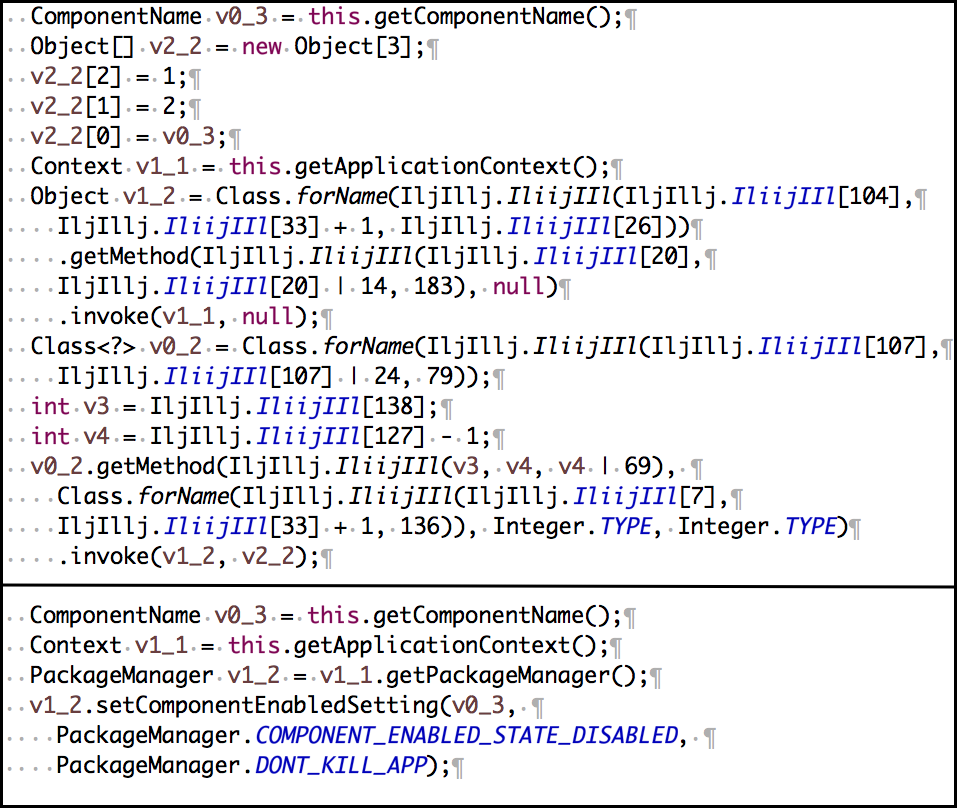
\includegraphics[width=3.5in]{fig/obadCodeSnippet.png}
\vspace{-.05in}
\caption{Obad Code Snippet. The obfuscated code is on the top; 
the de-obfuscated version is at the bottom.}
\label{fig:obadCodeSnippet}
\vspace{-.15in}
\end{figure}


One notable family that extensively adopts renaming and string encryption
techniques is \fn{Obad}.
Figure~\ref{fig:obadCodeSnippet} shows the code snippets
in \fn{Obad} and the corresponding translation.
We can see that, the obfuscation renames all classes, methods, fields to 
human unreadable forms (\eg {\em IljIllj}, {\em IliijIIl}, \etc).
Furthermore, all invoke statements
in the unobfuscated bytecode are translated to java reflection in the obfuscated version, 
and the name strings of such reflection are further encrypted and stored in a byte array 
list ``IliijIIl.''
The decrypting method ``{\em IljIllj.IliijIIl}'' takes the byte array from ``IliijIIl'' and
decrypts it and makes the reflection call.
This clearly shows that the obfuscation can make both manual analysis
and static analysis extremely difficult.

%\ptitle{Dynamic Loading (DL)}

{\bf Dynamic Loading} dex file becomes more popular nowadays. 
Normally it contains a dropper payload, which is lightweight
and looks benign.
But this dropper payload will then load the real
payload from its assets or resource folder (\eg \fn{RuMMS}), 
or download the real payload from internet (\eg \fn{SlemBunk}).
To further complicate the analysis, the real payload can even be encrypted (\eg \fn{Fobus}).

%\ptitle{Native Payload (NP)}

{\bf Native Payload}: Most of the static analysis tools focus on Dalvik bytecode.
So the native
library seems to be a good place to hide malware behavior.
In our analysis, we observed that native payloads are becoming
more popular. Malware apps not only hide functionalities,
but also hide sensitive strings, like server URL, premium numbers in the native code.
%\fn{xxx} hides the sms aborting logic in the native payload whereas
%\fn{Ogel} hides the url in the native payload.

%\ptitle{Evade Dynamic Analysis (EDA)}

% On the other hand, cybercriminals invented many ways to evade dynamic analysis.
{\bf Evade Dynamic Analysis}: The basic idea of evading dynamic analysis is to detect the malware's
current running environment.
For example,
when \fn{BankBot} \cite{bankBot} gets activated, it will check whether
IMEI, MODEL, FINGERPRINT, MANUFACTURE, BRAND and DEVICE are of certain
value.
%\begin{itemize}[noitemsep]
%\item Is {\em IMEI} equals ``000000000000000"?
%\item Is {\em Build.MODEL} contains ``google_sdk", ``Emulator", ``Android SDK", or ``Android SDK built for x86"?
%\item Is {\em Build.FINGERPRINT} starts with ``generic" or ``unknown"?
%\item Is {\em Build.MANUFACTURER}  contains ``Genymotion"?
%\item Is {\em Build.BRAND} starts with ``generic"?
%\item Is {\em Build.DEVICE} starts with ``generic"?
%\end{itemize}
If the running environment satisfies the condition,
it will act benignly and stop itself.
\fn{Triada} will check if IMEI matches some pattern, and
check whether ``com.qihoo. androidsandbox'' is installed.
To thwart dynamic analysis that monitors the communication
channel (\eg Internet, SMS.) of the malware,
many malware encrypt communication with their C\&C servers.

Many of these anti-analysis techniques involve encryption;
thus how to obtain the key is important to the analyst.
In most of the cases, the key is just hardcoded in the application code.
Some malware put the key in the
manifest, a resource XML file, or in the native payload.
We also observed a few smart ways to hide or generate the keys.
\fn{Fobus} reads the JVM stack trace and uses the class and method name
of the fourth entry in the stack to construct the key. 
\fn{Obad} obtains its key by requesting a webpage from Facebook, and reads
certain location from that webpage to generate the key.

%%% Local Variables: 
%%% mode: latex
%%% TeX-master: "paper"
%%% End: 

\vspace{-.1in}
\subsection{Monetization}
\label{sec:profile:monetize}
\vspace{-.1in}

% Malware apps are evolving over the usage of monetization techniques. 
We observe that many malware attempt to make money from the victims
as Table~\ref{table:monetization} illustrate.

\begin{table}[!t]
\centering
\scriptsize
\caption{Monetization Techniques.}
\label{table:monetization}
\begin{subtable}{0.495\textwidth}
\centering
\scriptsize
\resizebox{\textwidth}{!}{ %
\begin{tabular}{?p{2.3cm}|c|c|c|c?}
\Xhline{2\arrayrulewidth}
\multirow{2}{*}{Family} & Premium Service & \multirow{2}{*}{Bank} & \multirow{2}{*}{Ransom} & Aggressive \\
				      & Subscription	    &					&					& Advertising \\
\hline
\hline
Airpush & Dynamic &  &  & \checkmark \\
\hline
AndroRAT & Dynamic &  &  &  \\
\hline
Andup &  &  &  & \checkmark \\
\hline
Aples &  &  & \checkmark &  \\
\hline
BankBot &  & \checkmark &  &  \\
\hline
Bankun &  & \checkmark &  &  \\
\hline
Boqx &  &  &  &  \\
\hline
Boxer & Static &  &  &  \\
\hline
Cova & Dynamic\&Static &  &  &  \\
\hline
Dowgin &  &  &  & \checkmark \\
\hline
DroidKungFu &  &  &  &  \\
\hline
Erop & Static &  &  &  \\
\hline
FakeAV &  &  & \checkmark &  \\
\hline
FakeAngry &  &  &  &  \\
\hline
FakeDoc & Static &  &  &  \\
\hline
FakeInst & Dynamic\&Static &  &  &  \\
\hline
FakePlayer & Static &  &  &  \\
\hline
FakeTimer &  &  &  &  \\
\hline
FakeUpdates &  &  &  &  \\
\hline
Finspy &  &  &  &  \\
\hline
Fjcon & Dynamic &  &  &  \\
\hline
Fobus & Dynamic &  &  &  \\
\hline
Fusob &  &  & \checkmark &  \\
\hline
GingerMaster &  &  &  &  \\
\hline
GoldDream & Dynamic &  &  &  \\
\hline
Gorpo &  &  &  & \checkmark \\
\hline
Gumen & Dynamic &  &  &  \\
\hline
Jisut &  &  & \checkmark &  \\
\hline
Kemoge &  &  &  &  \\
\hline
Koler &  &  & \checkmark &  \\
\hline
Ksapp &  &  &  &  \\
\hline
Kuguo &  &  &  & \checkmark \\
\hline
Kyview &  &  &  & \checkmark \\
\hline
Leech &  &  &  & \checkmark \\
\hline
Lnk &  &  &  &  \\
\hline
Lotoor &  &  &  &  \\
\hline
Mecor &  &  &  &  \\
\Xhline{2\arrayrulewidth}
\end{tabular}
}
\end{subtable} %
\begin{subtable}{0.495\textwidth}
\centering
\scriptsize
\resizebox{\textwidth}{!}{ %
\begin{tabular}{?p{2.3cm}|c|c|c|c?}
\Xhline{2\arrayrulewidth}
\multirow{2}{*}{Family} & Premium Service & \multirow{2}{*}{Bank} & \multirow{2}{*}{Ransom} & Aggressive \\
				      & Subscription	    &					&					& Advertising \\
\hline
\hline
Minimob & Dynamic &  &  & \checkmark \\
\hline
Mmarketpay & Dynamic &  &  &  \\
\hline
MobileTX & Static &  &  &  \\
\hline
Mseg & Dynamic &  &  &  \\
\hline
Mtk &  &  &  &  \\
\hline
Nandrobox & Static &  &  &  \\
\hline
Obad & Dynamic &  &  &  \\
\hline
Ogel &  &  &  &  \\
\hline
Opfake & Dynamic\&Static & \checkmark &  &  \\
\hline
Penetho &  &  &  &  \\
\hline
Ramnit &  &  &  &  \\
\hline
Roop &  &  & \checkmark &  \\
\hline
RuMMS & Dynamic & \checkmark &  &  \\
\hline
SimpleLocker &  &  & \checkmark &  \\
\hline
SlemBunk &  & \checkmark &  &  \\
\hline
SmsKey & Static &  &  &  \\
\hline
SmsZombie &  & \checkmark &  &  \\
\hline
Spambot & Static &  &  &  \\
\hline
SpyBubble &  &  &  &  \\
\hline
Stealer & Dynamic &  &  &  \\
\hline
Steek &  &  &  &  \\
\hline
Svpeng & Dynamic & \checkmark & \checkmark &  \\
\hline
Tesbo &  &  &  &  \\
\hline
Triada & Dynamic & \checkmark &  &  \\
\hline
Univert & Dynamic &  &  &  \\
\hline
UpdtKiller & Dynamic &  &  &  \\
\hline
Utchi &  &  &  & \checkmark \\
\hline
Vidro & Dynamic &  &  &  \\
\hline
VikingHorde &  &  &  & \checkmark \\
\hline
Vmvol & Dynamic &  &  &  \\
\hline
Winge & Dynamic &  &  &  \\
\hline
Youmi &  &  &  & \checkmark \\
\hline
Zitmo &  & \checkmark &  &  \\
\hline
Ztorg &  &  &  & \checkmark \\
\Xhline{2\arrayrulewidth}
Total families: & 30 & 9 & 8 & 12  \\
\hline
Total varieties: & 41 & 27 & 13 & 13  \\
\hline
Total apps: & 11839 & 1652 & 2166 & 14336  \\
\Xhline{2\arrayrulewidth}
\end{tabular}
}
\end{subtable}
\end{table}

\vspace{-.15in}
\subsubsection{Premium Service Subscription}
\label{sec:profile:monetize:premium}

Subscribing to a premium service is one of the main ways
cybercriminals use to make money.
In general, subscribing to a premium service
requires the malware app to send a request to the service provider.
The premium service sends back a confirmation
message, which has to be entered back
to finish the subscription process.
A comprehensive premium-service-subscription module includes
a premium service requester and an incoming message handler.
% The requester is responsible for obtaining
% The premium service phone numbers or urls are either hard-coded
% in the binary ({\bf Static}) or fetched from C\&C server at run-time ({\bf Dynamic}).
The service requester makes phone calls, sends SMS or network request to the premium service.
After that, the malware waits for the services to reply with confirmation message.
The incoming message handler intercepts the confirmation message and
parses it. It then applies a handler logic
based on different subscription routines,
and cleans any evidence that might alert the victim user.

In our analysis, we found the following ways to obtain the premium numbers
and handler logic: hard coded into the bytecode,
hidden in the resource XML files or native library,
encrypted, and dynamically configured from C\&C server.

% Let us take two examples.
% (1) \fn{Boxer} loads and decrypts resource files
% from the asset folder that
% contains information about the app owner's email,
% update url, country code with
% premium numbers and message text.
% It then reads country code from the device, and chooses
% corresponding premium numbers to send subscription
% messages.
% (2) \fn{Fobus} sends an HTTP request for a paid web content.
% The paid web service will reply with an SMS message
% with a PIN code to the requester.
% The malware captures the SMS and automatically reply with the
% PIN code to the web service.
% Some of the paid web services require the requester to resolve
% a CAPTCHA challenge. In that case, the malware will upload such
% challenge picture to antigate.com,
% which is a real-time captcha-to-text decoding web service.
% After the challenge is resolved, it will automatically submit it 
% to the paid web service.

\subsubsection{Banking Trojan}
\label{sec:profile:monetize:bank}

\begin{figure}[t]
\centering
\begin{minipage}{.5\textwidth}
  \centering
  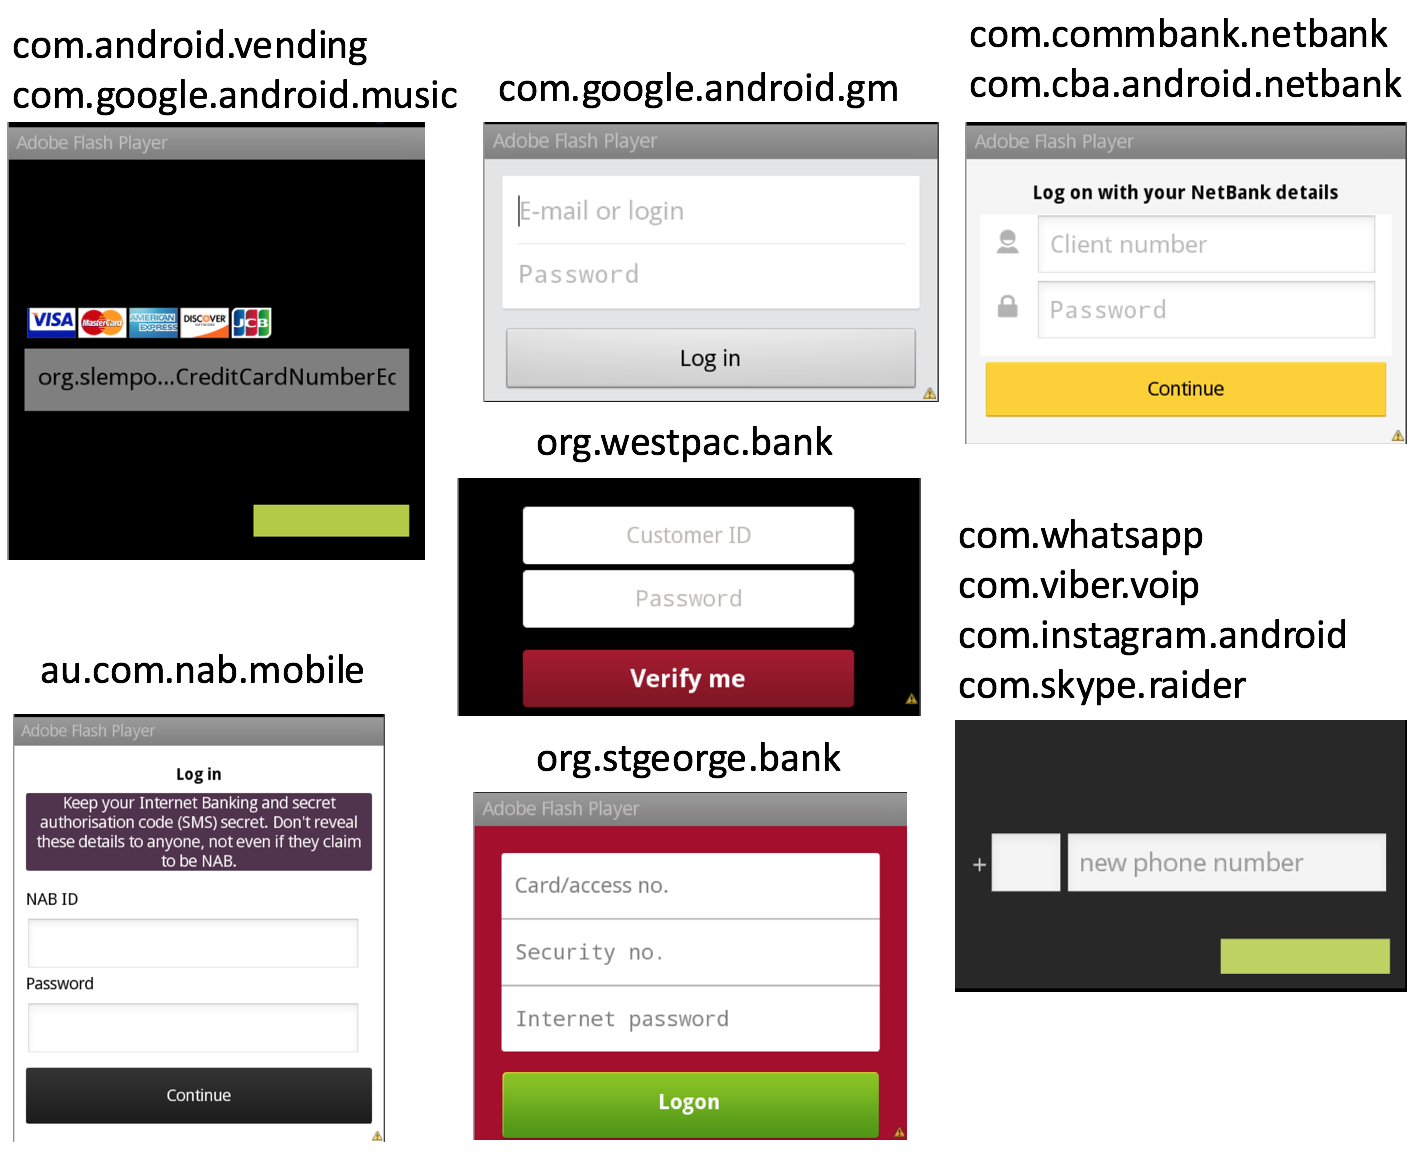
\includegraphics[width=2in]{fig/slembunkWindows.png}
  \captionof{figure}{Slembunk Phishing Windows}
  \label{fig:slembunkPhishingWindows}
\end{minipage}%
\begin{minipage}{.5\textwidth}
  \centering
  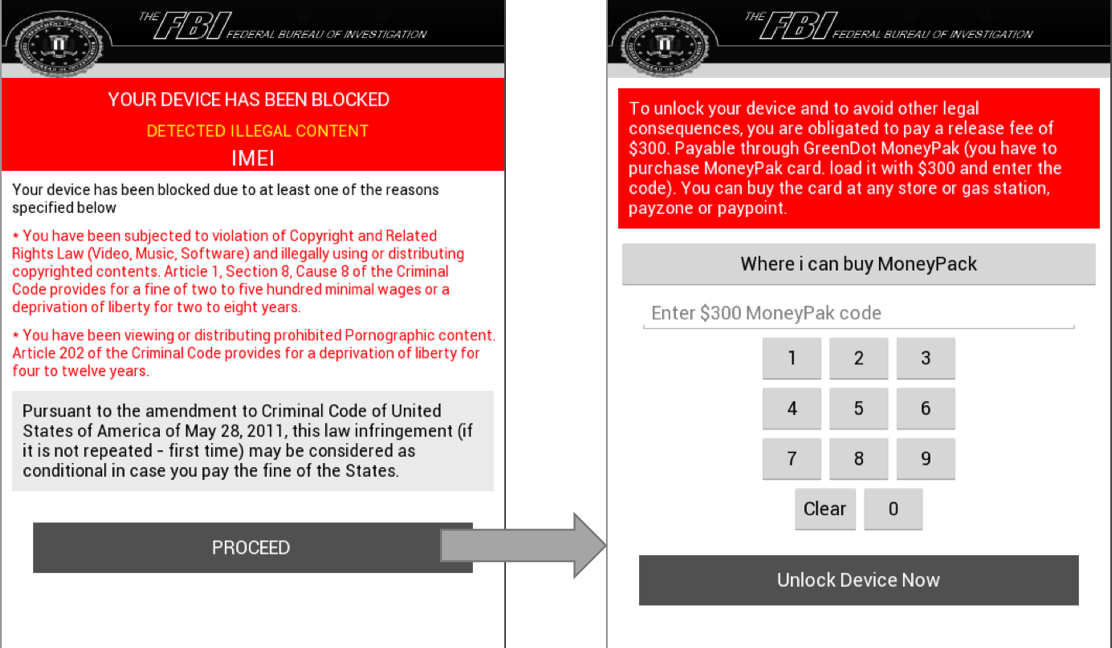
\includegraphics[width=2.35in]{fig/apleswindow.png}
  \vspace{.22in}
  \captionof{figure}{Ransom Windows by Aples}
  \label{fig:apleswindow}
\end{minipage}
\end{figure}

% Banking activities are associated with people's daily life.
Online payment and mobile wallet are becoming more popular nowadays.
Cybercriminals are also putting much effort to increase their revenue
by designing banking trojans.
%The early-stage mobile banking trojans, \eg \fn{Zitmo} work in
%combination with windows-based trojans
%to capture mTAN passwords (one-time password
%used in two-factor authentication).
In 2013, banking trojan \fn{Bankun} came into picture.
Once activated this trojan will check the 
compromised device for installed Korean banking applications,
and try to replace them with fake ones. 
%It does so by showing the victim user
%messages like ``a critical update is available for a banking app'' or
%``update is required right now.''
%The fake banking apps are well designed and look exactly the same as
%the original one. But once the user types in the banking credential,
%it will be uploaded to the cybercriminal's server.
Newer versions of banking trojans are capable of overlaying the
on-screen display of a legitimate banking app with a phishing
window.
\fn{Slembunk} falls into this category.
When this malware is activated, it will
schedule a {\em java.lang.Runnable} every 4 seconds to monitor
the current running applications by looking at the Activity
at the top of the Activity stack.
If the current running Activity belongs to certain banking
application, it will overlay a phishing window on top of the screen.
Figure~\ref{fig:slembunkPhishingWindows} shows what the phishing window
looks like for different banking applications. As an example,
if the current application is {\em com.android.vending} the left top window will be popped, and so on.
\fn{Slembunk} not only overlays phishing windows,
it is also capable of forwarding phone calls and SMS from bank
numbers, and applying the response logic.
To effectively conceal the arrival of text messages or phone calls from banks,
it will mute the device's audio system.
Later versions of \fn{Slembunk} even apply most sophisticated
string encryption and dynamic loading obfuscation techniques
(Section~\ref{sec:profile:behavior:anti}).
Recently, IBM and FireEye report~\cite{sourceCodeLeakedFireeye,sourceCodeLeakedIBM} that
the source code of \fn{SlemBunk} was leaked, which
could result in the emergence of more variants.

\vspace{-.15in}
\subsubsection{Ransom}
\label{sec:profile:monetize:ransomware}

Ransomware % is a kind of malware which is capable
locks the victim device by making it
non-responsive or encrypting its data, and
then coerces the victim to pay for the restoration.

\ptitle{Device Locking Techniques}

%\fn{FakeAV} is a fake anti-virus software.
%When it starts running, it pretends to scan victim's device.
%No matter the device is infected by malware or not,
%it will randomly choose some malware description from its database,
%and will intimidate the victim that her device is compromised,
%and to stay safe, the victim has to buy the pro version.
%If the victim keeps using the free version,
%it will use {\em AlarmManager} to periodically
%schedule a {\em BroadcastReceiver},
%which will notify the victim that the device is compromised.
%Furthermore, it will monitor victim's SMS and phone call,
%and also alerts the victim that there are viruses in the SMS or
%phone conversation is not protected.

%\begin{figure}[t]
%\centering
%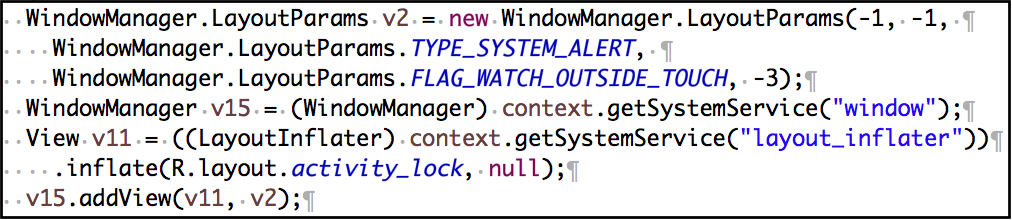
\includegraphics[width=2in]{fig/svpengInflateCodeSnippet.png}
%\vspace{-.1in}
%\caption{Svpeng Lock Screen Code Snippet}
%\label{fig:svpengInflate}
%\vspace{-.2in}
%\end{figure}

\fn{Svpeng} is both a banking trojan and ransomware.
If its C\&C server sends a command ``forceLock,''
it will lock the infected device by using SYSTEM_ALERT_WINDOW
permission and {\em WindowManager LayoutParams} 
with certain flags (\eg FLAG_SCREEN, FLAG_LAYOUT_IN_SCREEN,
FLAG_WATCH_OUTSIDE_TOUCH, \etc)
to achieve an unremovable full screen floating window.
%Figure~\ref{fig:svpengInflate} shows how it looks like
%in the code.

\fn{Aples} first appeared in 2014 -- when activated, it will
schedule a {\em Runnable} in every 0.1 second
to load the threatening window
with flag FLAG_ACTIVITY_NEW_TASK
which looks like Figure~\ref{fig:apleswindow}.
Clicking on ``PROCEED'' at the first window
will lead to the second window that asks the victim user to fill in a 
\$300 MoneyPark code to unlock.
Another malware family \fn{SimpleLocker} has applied similar techniques,
at the same time also encrypting all the data in the compromised device's external
storage using AES with a hardcoded key.

\fn{Jisut} once activated will launch a ransom window, and override {\em onKeyDown}
method of {\em Activity} to redirect key press event (\eg return key, volume key, menu key, \etc)
to some meaningless action to achieve the lock screen purpose.

\vspace{-.05in}
\ptitle{Device UnLocking Techniques}

After the victim has paid the money, the cybercriminal will tell the victim 
how to unlock the device or unlock it remotely.
The most common way is to type in the pin. 
The pin in one variety of \fn{SimpleLocker} is generated by
obtaining a serial number at beginning (which is a random number),
then uses some calculation logic (in one sample, the logic is {\em key = (serial_number - 2016)*2 + 2016}).
The second way is using remote control.
For instance, \fn{Koler} uses network command to clear a lock tag at the malware's shared preference.
The third way is by installing an unlock app.
One variety of \fn{Jisut} constantly checks whether an app with package
``{\em tk.jianmo.study}'' is installed or not; if yes, it will release the lock.

\vspace{-.2in}
\subsubsection{Aggressive Advertising}
\label{sec:profile:monetize:adware}

Mobile advertising is the main revenue source for app developers as well as
malware writers. Advertising in malware is usually more aggressive,
and this kind of apps are called adware.

\vspace{-.05in}
\ptitle{Potentially Unwanted Application (PUA)} 
A PUA adware performs tasks such as monitoring victim's personal data,
showing unwanted advertisement content,
annoying victim user with aggressive advertisement push,
showing and tempting the victim to download and install potential harmful applications.
\fn{Dowgin} is one adware app.
It will be activated once the device connectivity changes, 
user comes into presence,
or a new application is installed or deleted.
Once activated, it will display unwanted advertisements in the system's notification bar.
If the victim clicks on this notification, it will show an application wall which attracts
the victim to install new applications.
At the same time, it will send device information and the list of installed apps to a remote
C\&C server using JSON, and receive commands for showing a new advertisement,
uploading client info \etc
Many other adwares have similar behaviors, \eg \fn{Airpush}, \fn{Kuguo}, \fn{Youmi}.

\ptitle{Malware Dropper}
% A few newly found (after 2015) adware families%  try to leverage
% % root privilege and
% drop malware siliently on the infected device.
% so they are also called malware droppers.
\fn{Gorpo}, \fn{Kemoge} \cite{kemoge}, \fn{Leech} and \fn{Ztorg} are some examples.
Their task is to gain the root privilege on the infected device as discussed in 
Section~\ref{sec:profile:behavior:privilege}, and then silently drop all the active 
malware apps that are available on the ``malvertising campaign network'' to the infected device.
\fn{VikingHorde} is running in two modes: rooted and not-rooted.
If the device is not rooted, it performs in a regular fashion: uploading victim's data, 
fetch command from C\&C to execute, \etc
If the device is rooted, it will install some additional components, which are capable of 
constantly and silently downloading new malware onto the device.
We include this as part of aggressive advertising even though their main purpose
is spreading malware.

%%% Local Variables: 
%%% mode: latex
%%% TeX-master: "paper"
%%% End: 


%%% Local Variables: 
%%% mode: latex
%%% TeX-master: "paper"
%%% End: 

\vspace{-.15in}
\section{Evolution}
\label{sec:evolution}
\vspace{-.1in}

\begin{figure}[t!]
\centering
\begin{subfigure}[b]{.32\textwidth}
  \centering
  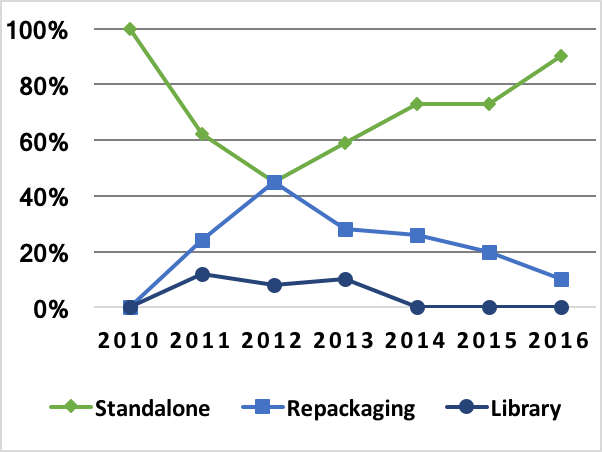
\includegraphics[width=0.9\linewidth]{fig/charts/comp.png}
  \caption{Composition}
  \label{fig:sub:ins}
\end{subfigure}%
\begin{subfigure}[b]{.32\textwidth}
  \centering
  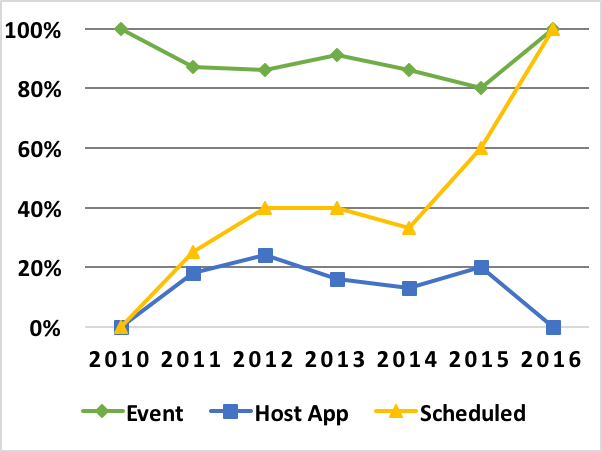
\includegraphics[width=0.9\linewidth]{fig/charts/act.png}
  \caption{Activation}
  \label{fig:sub:act}
\end{subfigure}%
\begin{subfigure}[b]{.32\textwidth}
  \centering
  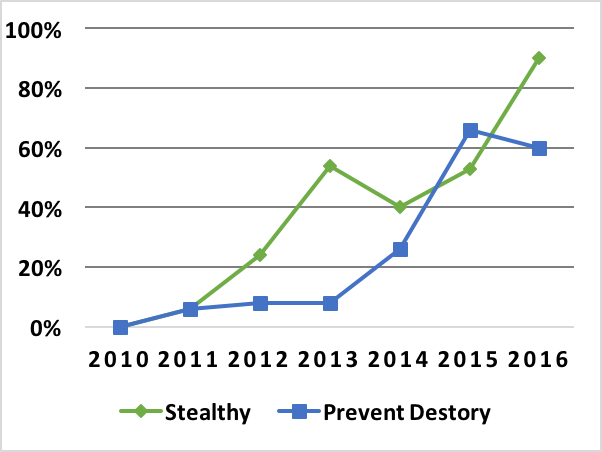
\includegraphics[width=0.9\linewidth]{fig/charts/per.png}
  \caption{Persistence}
  \label{fig:sub:per}
\end{subfigure}
\begin{subfigure}[b]{.32\textwidth}
  \centering
  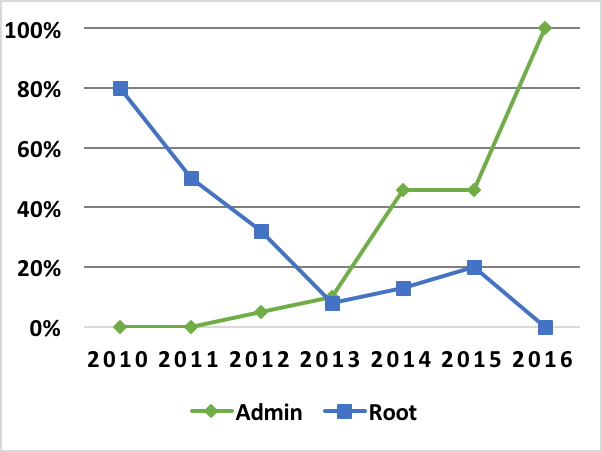
\includegraphics[width=0.9\linewidth]{fig/charts/pri.png}
  \caption{Privilege}
  \label{fig:sub:pri}
\end{subfigure}%
\begin{subfigure}[b]{.32\textwidth}
  \centering
  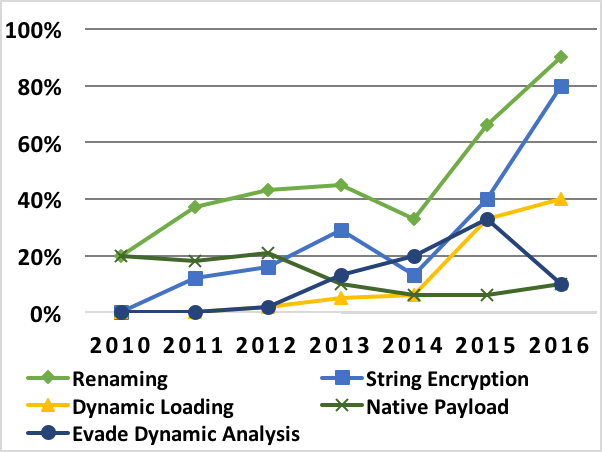
\includegraphics[width=0.9\linewidth]{fig/charts/anti.png}
  \caption{Anti-analysis}
  \label{fig:sub:anti}
\end{subfigure}%
\begin{subfigure}[b]{.32\textwidth}
  \centering
  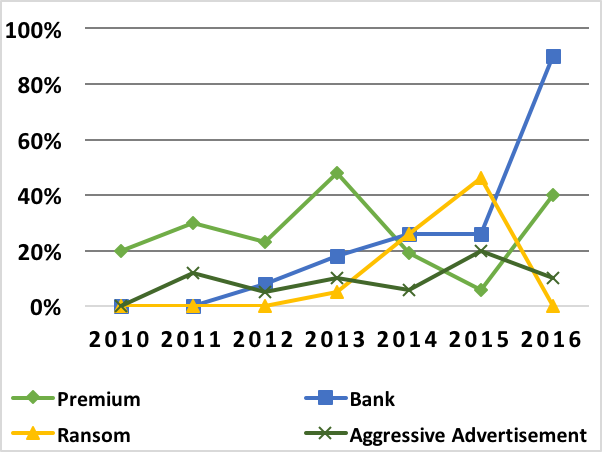
\includegraphics[width=0.9\linewidth]{fig/charts/mone.png}
  \caption{Monetizing}
  \label{fig:sub:mono}
\end{subfigure}
\caption{Malware Behavior Trends %. X axis represents the year from 2010 to 2016 whereas 
% (Y axis shows percentage within the year)  of malware variants appearing within the year
% having a particular behavior.
}
\vspace{-.25in}
\label{fig:behaviorcharts}
\end{figure}

We have performed a longitudinal study of our malware dataset with an attempt
to discover the trend of malware behaviors and techniques used over the years
from 2010 to 2016. For each type of behaviors and techniques, 
we observe the trend in terms of percentage of malware varieties manifesting a specific 
behavior/technique within a year.
%  requesting device-admin-privilege compared to percentage of malwares
% with root-exploit over the years).
Figure~\ref{fig:behaviorcharts} presents the results.
% evolution trace of the malware behavior and techniques.

Figure~\ref{fig:sub:ins} shows that the repackaging usage was growing until 2012,
but later standalone malware became dominant. The reason could be that
there are many effective anti-repackaging solutions made available during the last few years, 
which gives cybercriminals less incentive to use such techniques.
On the other hand, the bad guys are putting more effort into designing comprehensive
and sophisticated malware apps from scratch, and their malware design skill has matured. 

Not surprising to see in Figure~\ref{fig:sub:act} that listening to system events to
activate malware's functional units is the main trick given the nature of Android system design.
%Activation via host app comes along with repackaging or adware as expected.
Scheduling a task to periodically start its functional unit is an alarmingly growing trend.
By scheduling timer task or leveraging the {\em AlarmManager} the malware can constantly
upload victim's information to or retrieve commands from the C\&C server;
in the ransomware apps, it is also one of the techniques to lock victim's device.

We observe that persistence has become a core feature of Android malware apps. 
Figure~\ref{fig:sub:per} shows that malware apps are evolving to be harder 
to notice by the victim, % as they are hiding their appearance and hiding or cleaning the evidence.
and harder to be destroyed by the system,
anti-virus solutions, or users.

Root exploit is becoming less popular as we have discussed in Section~\ref{sec:profile:behavior:privilege},
but obtaining device-admin-privilege seems to have become popular as seen in Figure~\ref{fig:sub:pri}.
% We think that is because admin-privilege not only makes it harder to be uninstalled,
% but also can give cybercriminals the power to threat the victim user that her
% data is in danger.

The anti-analysis techniques are one of the key weapons of cybercriminals in 
the battle against security analysts.
From Figure~\ref{fig:sub:anti} we can see that renaming and string encryption
are the most growing techniques;
dynamic loading and evading dynamic analysis are catching up while
the practice of hiding behaviors in native payload is staying at the similar level.

Figure~\ref{fig:sub:mono} shows that banking malware is becoming the 
main channel for cybercriminals to make money.
% This is because people's banking behaviors are migrating from the
% PC world to the mobile phones, and more and more financial related activities are becoming available on mobile devices.
%Subscribe to premium service remains the same over the years.
Ransomware is a new threat that has started an uptick.

%%% Local Variables: 
%%% mode: latex
%%% TeX-master: "paper"
%%% End: 

%\section{Finding Summary}
\label{sec:value}

We provide the community a well-labeled Android malware dataset
that includes comprehensive profile information about malware behaviors
and techniques. The dataset provides an up-to-date picture of
the current landscape of Android malware. 
% Our study strongly suggests that \genome dataset is
% outdated as it does not capture most of the current malware
% behaviors. Our observations warrant an urgent need for a new dataset to better
% guide the design of new Android anti-virus solutions.
Below we highlight the main findings we obtained from analyzing the
malware samples in our dataset.

\begin{enumerate}[leftmargin=0cm,itemindent=.5cm,labelwidth=\itemindent,labelsep=0cm,align=left]

\item Android malware monetizing techniques are evolving.
% To better understand the landscape of Android malware,
We need to understand the way cybercriminals generate revenue
for more effective malware analysis and prevention.
% The malware design is dictated by how to steal money 
% and how to keep the malware alive longer,
% so if we perform the analysis along this line, we can
% get more clear picture of the Android malware world.

\item We observe that \emph{standalone} malware apps
are becoming dominant. This indicates that the Android security community
did a good job of capturing repackaged malware, but it also
gives us a message that the war against Android malware has escalated to another stage,
where cybercriminals are becoming more skilled and putting
more effort into designing more comprehensive and sophisticated malware.
% Android ecosystem is growing fast with more and more features being added
% and more financial related activities becoming available.
% This means that Android malware will not stop evolving, so
% anti-virus solutions also have to catchup to guard against the threats.

\item Malware writers are more aggressively using persistence techniques in the malware design.
% Assuming mobile device users care about the security issues of their device,
% any suspicious behavior will alarm the users about existence of a malware.
% So to make the malware stay longer on the infected device, leaving less evidence
% is the key of success for a malware app.

\item Anti-analysis techniques are being widely used in Android malware these days,
and the obfuscation techniques make malware analysts job much harder. % The
% dynamic analysis evading techniques are used to hide the malicious behavior from the
% dynamic vetting sandbox.
When the detection of malware
becomes harder, the malware gets larger time window to exist on the wild harming victims.
This shows an urgent need of designing effective deobfuscation solutions. The 
dynamic analysis tools also need to keep up with evading techniques.
%  obfuscate more its environment to make it more
% like a normal device.

\end{enumerate}

%%% Local Variables: 
%%% mode: latex
%%% TeX-master: "paper"
%%% End: 

%\section{Discussion}

\subsection{Answering Research Questions}
\subsubsection{RQ1}
Do the popular DFR tools (as available in the market) meet the NIST CFTT standards? 
If not, which tool meets which part of the standard? 

Generally, we found that the DFR tools we tested did not meet the NIST CFTT standards.
Testdisk\cite{testdisk} failed to fulfill core feature 1 because it did not identify deleted files in two test cases.
All tools fulfilled core feature 2, as they produced a recovered object for every deleted file they identified.
Autopsy\cite{autopsy} and Magnet AXIOM\cite{axiom} failed to fulfill core feature 3 because in several test cases they did not recover data they had access to.
All tools failed to fulfill core feature 4 because in many cases they recovered data which was not part of the original file.

\subsubsection{RQ2}
What factors make the tools fail or succeed?

The most common factor causing tools to fail is when a deleted file has been overwritten.
Core feature 4 requires that a tool only recover data which was originally a part of the deleted file.
A tool's success regarding this feature is thus a measure of its restraint.
The only tool to consistently fulfill core feature 4 is FTK Imager.\cite{ftk}
When it detects that a file has been partially or completely overwritten by another file, it omits the deleted sections (and everything after them in FAT).
However, in cases when the overwriting file has also been deleted, even FTK fails to fulfill this core feature.
It is worth noting that Autopsy does appear to react to overwritten files; for some cases of overwriting in FAT, it returns only a single cluster, presumably the starting cluster of the deleted file.
However, since that cluster has been overwritten, Autopsy still fails to fulfill core feature 4 in those cases.

Another factor that causes multiple failures is simulated in FAT cases 8, 9, and 10.
In FAT, a file can be written starting close to the end of the file system, without enough space to fit contiguously.
In such cases, the file must be fragmented, and since it is already at the end of the file system, the second fragment will appear closer to the beginning of the file system (this is illustrated in Figure \ref{fig:case_8}).
This scenario could realistically occcur when the file system is almost full.
In these cases, no tool is able to recover the second fragment of the deleted file; however, because FAT fragmentation is unpredictable, we only require them to recover the first fragment.
Interestingly, Autopsy and Magnet AXIOM fail to recover anything at all, with Autopsy returning a short file of null data, and Magnet AXIOM returning an empty file after displaying an error message.

\subsubsection{RQ3}
Are the free DFR tools more effective compared to the enterprise-level (proprietary) tools?

As can be observed in Figure \ref{table:results_table}, no type of tool clearly outperforms the others.
FTK Imager, a proprietary enterprise-level tool, passes the most test cases by a large margin.
However, the other enterprise-level tool, Magnet AXIOM, passes the least test cases.
Given the available data, we cannot reach a definite conclusion for RQ3.

\begin{table}[h!]
    \caption{DFR tools sorted by type. ``Passes'' refers to the number of test cases in which a tool fulfills all 4 core features.}
    \label{table:results_table}
    \begin{tabular}{| c | c | c |}
    \hline
    \textbf{DFR Tool} &  \textbf{Type} &  \textbf{Passes} \\ \hline
    Autopsy & free open source & 5 \\ \hline
    TestDisk & free open source & 10 \\ \hline
    Recuva & proprietary freemium & 7 \\ \hline
    FTK Imager & proprietary enterprise & 18 \\ \hline
    Magnet AXIOM & proprietary enterprise & 4 \\ \hline
    \end{tabular}
\end{table}    

\subsection{Ambiguity in Standards}
While determining how to interpret the NIST standards, we encountered ambiguities in their current wording.

\subsubsection{Core Feature 3 and FAT Fragmentation}
Core feature 3's requirement that a tool recover ``all non-allocated data blocks identified in a residual metadata entry''\cite{meta:dfr:standards} is not well-defined when considering a FAT file system. 
In FAT, the only relevant metadata left over after file deletion is the address of the first cluster of file data, and the file's length. 
If the deleted file is fragmented at any point, no evidence remains in the metadata. 
Therefore, interpreting the wording very closely, a tool is only required to recover the first cluster of a file's data. 
As this would not be particularly useful, it is unlikely that this was the intended meaning. 
For these tests we interpret core feature 3 as requiring the first contiguous segment of unallocated clusters starting from the first cluster originally allocated to the deleted file. 
In other words, if the file is fragmented, the tool must recover at least the first fragment. 
If a file is partially overwritten, the tool must recover at least the clusters before the overwritten part.
In essense, the tool is only required to recover data for which it does not have to guess what file the data belongs to.
However, it should be emphasized this is an assumption and the intent of the standard in this case needs clarification.

\subsubsection{Contradictory Core Features}
When designing test cases, we found situations in which core features 3 and 4 are entirely incompatible. 
Core feature 3 specifies ``all non-allocated data blocks identified in a residual metadata entry,''\cite{meta:dfr:standards} but that can sometimes still include data from other files. 
One such situation is when a deleted file is overwritten, and then the overwriting file is also deleted, such as in case 5i (as seen in Figure \ref{fig:case_5i}).

\begin{figure}[h]
    \centering
    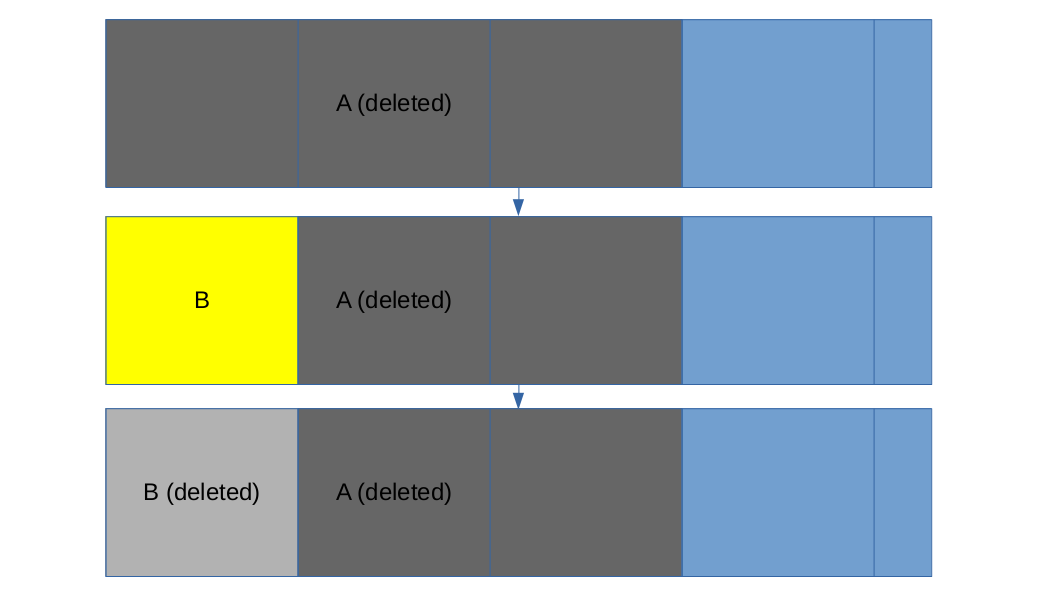
\includegraphics[width=\linewidth]{fig/case5i.png}
    \caption{Test Case 5i}
    \label{fig:case_5i}
\end{figure}

Assuming the file system is NTFS (to avoid the afforementioned ambiguity with core feature 3 and FAT), the residual metadata entry for File A (in this case its Master File Table entry) should list every cluster File A once occupied. 
All of those clusters are unallocated, so to fulfill core feature 3, the tool must recover them. 
However, some of those clusters have been overwritten by File B. Core feature 4 requires that a tool only recover ``data blocks from the Deleted Block Pool,''\cite{meta:dfr:standards} and defines the Deleted Block Pool as all blocks which ``have not been reallocated or reused.''\cite{meta:dfr:standards}
Core feature 3 would require tools to recover the clusters reused by File B, while core feature 4 would forbid this. 
It could be argued that the tool should use File B's metadata to recognize that File B overwrote File A, but this is not always realistic. 
While the file system stores information such as creation and modification times, this is not ``essential metadata,'' meaning it is not involved in the operation of the file system, so operating systems may implement it inconsistently, or not at all.\cite{carrier:filesystems}
Since the time information cannot be counted on to be reliable, there is no way to know for sure which file overwrote which. 
It is also possible for File B's metadata entry to be overwritten at some point before File A's, in which event there is no way for the tool to know File B even existed.

The standards document acknowledges that the ``potential for corruption [is] inherent with data that is no longer maintained by a file system,''\cite{meta:dfr:standards} and that the recovered object ``may not completely match the original FS-Object.''\cite{meta:dfr:standards}
We propose the standards themselves should be revised to better account for such situations.
This would most likely mean adding an exception to either the third or fourth core feature, for cases in which data blocks are overwritten and subsequently deallocated.

\subsection{Future Work}
The NIST CFTT standard includes several optional features; these features could be explored using a similar methodology.
We only created test images for the FAT and NTFS filesystems; our process could be expanded to other common filesystems such as ext4 and HFS.
NIST CFTT has a separate set of standards for file carving DFR tools; future work could involve creating test cases for file carving tools.

\vspace{-.1in}
\section{Related Work}
\label{sec:related}
\vspace{-.02in}

The \genome~\cite{zhou2012dissecting} %  is the closest related work of the current paper. 
% This
was the first research project that has provided the community 
an Android malware dataset. 
%In particular, it contains 1260 malware apps categorized in 49 families, which were discovered in 2010 and 2011. 
This dataset has been the only well-labeled one and has been widely studied 
and used by the research community.
Unfortunately, it has not been updated after its creation time around 2011.
We comparatively studied this dataset with the new malware samples we have, 
and found that the Genome dataset does not include many of the new threats, 
which motivated us to carry out this work. Our dataset also provides much more
detailed information on Android malware behaviors than that in Genome. Moreover,
we provide detailed documentation of the process used in creating the dataset, 
including the guidelines for the manual analysis, to help other researchers
do the same.
%In short, Genome dataset no longer represents the current Android malware world, which has motivated us to do the current work. 

Recently, the \emph{AndroZoo}~\cite{allix2015androzoo} dataset has been published, 
which contains more than 3 million Android apps 
from Google Play, other smaller markets, and app repositories.
\emph{AndroZoo}'s goal is to create a comprehensive app collection for software 
engineering studies. Our goal is different and we focus on (only) malware apps 
to study their security related behaviors. Our dataset provides malware labels
and detailed behavior information of the malware. 
% As expected, the majority of the apps in \emph{AndroZoo} are benign apps. 
% \emph{AndroZoo} did not yet report the behaviors of the malware apps in their dataset. 

There are a few other repositories for Android malware apps 
which researchers can use, such as \emph{Contagio Minidump}~\cite{minidump} 
and \emph{VirusShare}~\cite{virusshare}. However, they do not provide 
a comprehensive malware collection or comprehensive label and behavior information on
the malware.

The \emph{ANDRUBIS}~\cite{lindorfer2014andrubis} combines static and dynamic analysis
to automatically extract feature and behaviors from Android apps, and
studies the changes in the malware threat landscape and trends among ``goodware,'' or
benign apps, developers.
However, as many behaviors are either unknown or can evade the automated analysis method,
this work cannot give a comprehensive understanding of the malware landscape as we 
produced through the systematic and deep manual analysis.

\emph{AVclass}~\cite{sebastian2016avclass} provides a method to extract malware family name
by processing the AV labels obtained from VirusTotal. 
We adopted a similar approach for identifying malware family label.
Our work is focused on deep manual analysis of malware samples from different malware varieties, 
and reporting the detailed behavioral profiles for Android malware.

% independently developed without
% the knowledge of the AVclass work. The difference between own approach is discussed in
% Section~\ref{sec:data:family}. Furthermore, we provide the variety information for each malware family.

% Few recent works include \emph{Amandroid} \cite{wei2014amandroid}, \emph{DroidSafe} 
% \cite{gordon2015information}, \emph{FlowDroid} \cite{arzt2014flowdroid}, and \emph{IccTA} \cite{li2015iccta}.
% Future detection tools can utilize our malware dataset to test and improve the effectiveness. 

There has been quite some work on how to detect malicious apps. 
The \emph{Drebin}~\cite{arp2014drebin} work applies machine learning (ML) techniques to Android malware
detection.
The authors made the set of \emph{feature vectors} used in the ML work available to the community.
More recently, \emph{MassVet}~\cite{chen2015finding} provides a method
to detect malware apps by observing the repackaging traits (if any) 
compared to that of other apps. % However, \emph{MassVet} does not target other types (\ie standalone) 
% of malware.
Rastogi, \etal~\cite{rastogi2016these} conducted research on identifying adware tricks and drive-by-download techniques.
\emph{Harvestor}~\cite{rasthofer2016harvesting} attempts to extract the 
\emph{run-time} values from obfuscated apps
to detect malware. Researchers have identified ways in which Android users 
can be deceived to misidentify a malicious app window as a legitimate app's~\cite{bianchi2015app}.
Moreover, \emph{CopperDroid}~\cite{tam2015copperdroid} is a dynamic analysis system which attempts 
to reconstruct the behaviors of Android malware.
Our work complements these and other Android malware analysis work by providing a comprehensive 
dataset of Android malware with detailed label and behavior information, which can facilitate 
future research in this area.




%%% Local Variables: 
%%% mode: latex
%%% TeX-master: "paper"
%%% End: 

\vspace{-.1in}
\section{Conclusion}
\label{sec:conclusion}
\vspace{-.02in}

% We present a comprehensive analysis of the current landscape of Android malware.
% To help the research community better understand malware behavior
% and design new anti-virus solutions,
We created a large volume of well-labeled and well-studied
Android malware dataset containing \samsize samples, categorized in \versize
varieties among \fsize families ranging from 2010 to 2016.
For each variety of this dataset we 
conduct a comprehensive study to profile their behaviors and evolution trends.
We document in details the process of creating this dataset to enable other
researchers to replicate the process.
We observe that Android malware are evolving towards monetization, and becoming
sophisticated and persistent.
The extensive usage of anti-analysis techniques in the malware samples
shows the urgent need for advanced de-obfuscation and dynamic analysis methods.
We will make the dataset available to research community.

%%% Local Variables: 
%%% mode: latex
%%% TeX-master: "paper"
%%% End: 

\vspace{-.15in}
\section{Acknowledgment}
\label{sec:ack}
\vspace{-.05in}

This research is partially supported by the U.S. National Science Foundation under 
Grant No. 1622402. Any opinions, findings and conclusions or recommendations
expressed in this material are those of the authors and do not necessarily reflect 
the views of the National Science Foundation. This research is also partially supported by 
David and Amy Fulton Grant received by co-author Roy at Bowling Green State University.


%%% Local Variables:
%%% mode: latex
%%% TeX-master: "paper"
%%% End:


{\scriptsize
\bibliographystyle{plain}
\bibliography{android} 
}
%\appendix

%% \section{Appendix}
% \label{appendix}

The following tables present the malware families which appeared in the paper;
for the full table please refer to \amd.

\begin{table*}[!t]
\centering
\scriptsize
\vspace{-0.2in}
\caption{Malware Behaviors}
\label{table:behavior}
\vspace{-0.12in}
\begin{subtable}{1\textwidth}
\centering
\scriptsize
\resizebox{\textwidth}{!}{ %
\begin{tabular}{|l|l|l|l|l|l|l|l|}
\hline
\multicolumn{8}{|c|}{{\bf Legend}} \\
\hline
{\bf Installation} & Standalone (ST) & \multicolumn{3}{l|}{Repackaging (RPKG): Isolated (O), Integrated (T)} & Drop (DR) & Drive-by Download (DD) & Library (LIB) \\
\hline
{\bf Activation}  & Event (EV) & \multicolumn{2}{l|}{By Host App (BHA)} & Scheduling (SC) & {\bf Info Stealing} & Device Info (DI) & Personal Info (PI) \\
\hline
\multirow{2}{*}{\bf Persistence} & \multicolumn{1}{l}{Stealthy (TH):} & \multicolumn{6}{l|}{Block (BL), Clean (CL), Hide Icon (HI), Rootkit (RK)} \\
\cline{2-8}
                                                  &  \multicolumn{1}{l}{Prevent destroy (PD):} & \multicolumn{6}{l|}{Hide Admin (HA), Kill AV (KA), Lock Device (LD), Monitor Destroy Action (MDA), Reinstall (RI), System App (SYS)} \\
\cline{1-8}
{\bf Privilege} & Request Admin (RA) & \multicolumn{6}{l|}{Root Exploit (RE)} \\
\hline
{\bf C\&C} & Internet (IN) & \multicolumn{6}{l|}{Command Encoding (CE): Json (J), Java Script (JS), XML (X), Custom Protocol (P)} \\
\hline
\multirow{2}{*}{\bf Anti-analysis}  & Renaming (RN) & String Encryption (SE) & Dynamic Loading (DL) & \multicolumn{4}{l|}{Native Payload (NP)} \\
\cline{2-8}
                              & \multicolumn{7}{l|}{Evade Dynamic Analysis (EDA): Device Info (DI), Encrypt Communication (EC), Installed App (IA)} \\
\hline
\end{tabular}
}
\end{subtable}%

\begin{subtable}{1\textwidth}
\centering
\scriptsize
\resizebox{1\textwidth}{0.21\textheight}{ %
\begin{tabular}{?p{2.2cm}?c|c|c|c|c?c|c|c?c|c?c|c?c|c?c|c|c?c|c|c|c|c?}
\Xhline{2\arrayrulewidth}
\multirow{2}{*}{Malware} & \multicolumn{5}{c?}{Installation} & \multicolumn{3}{c?}{Activation} & \multicolumn{2}{c?}{Info Stealing} & \multicolumn{2}{c?}{Persistence} & \multicolumn{2}{c?}{Privilege} & \multicolumn{3}{c?}{C\&C} & \multicolumn{5}{c?}{Anti-analysis} \\
\cline{2-23}
 & ST & RPKG & DR & DD & LIB & EV & BHA & SC & DI & PI & TH & PD & RA & RE & IN & SMS & CE & RN & SE & DL & NP & EDA \\
\Xhline{2\arrayrulewidth}
Airpush &  &  &  &  & \checkmark &  & \checkmark & \checkmark & \checkmark & \checkmark &  &  &  & & \checkmark &  & J & \checkmark &  &  &  &  \\
\hline
AndroRAT & \checkmark &  & \checkmark &  &  & \checkmark &  & \checkmark & \checkmark & \checkmark &  &  &  & & \checkmark &  & P &  &  &  &  & \\
\hline
%Andup &  &  & \checkmark &  & \checkmark & \checkmark & \checkmark &  & \checkmark &  &  &  &  &  \\
%\hline
Aples & \checkmark &  &  &  &  & \checkmark &  & \checkmark & \checkmark &  &  & LD & \checkmark & & \checkmark &  & P &  &  &  &  & \\
\hline
BankBot & \checkmark &  & \checkmark & \checkmark &  & \checkmark &  & \checkmark & \checkmark & \checkmark & BL\&HI & MDA & \checkmark & & \checkmark & \checkmark & J\&P & \checkmark & \checkmark & \checkmark &  & DI \\
\hline
Bankun & \checkmark &  & \checkmark & \checkmark &  & \checkmark &  & \checkmark & \checkmark & \checkmark & BL\&HI &  & \checkmark & & \checkmark &  & J\&X &  &  &  &  & DI \\
\hline
%Boqx &  & O & \checkmark &  &  & \checkmark &  &  &  &  &  &  &  &  \\
%\hline
Boxer & \checkmark &  &  & \checkmark &  & \checkmark &  &  &  &  &  &  &  & &  &  &  & \checkmark & \checkmark &  &  &  \\
\hline
%Cova & \checkmark &  & \checkmark &  &  & \checkmark &  &  & \checkmark & \checkmark & BL &  &  &  \\
%\hline
Dowgin &  &  & \checkmark &  & \checkmark & \checkmark & \checkmark &  & \checkmark &  &  &  &  & & \checkmark &  & J & \checkmark & \checkmark & \checkmark &  & EC \\
\hline
DroidKungFu & \checkmark & O\&T & \checkmark &  &  & \checkmark & \checkmark & \checkmark & \checkmark & \checkmark &  & KA &  & \checkmark & \checkmark &  & J\&P & \checkmark & \checkmark &  & \checkmark & \\
\hline
%Erop & \checkmark &  &  &  &  & \checkmark &  &  & \checkmark &  &  &  &  &  \\
%\hline
FakeAV & \checkmark &  &  &  &  & \checkmark &  & \checkmark &  &  & BL &  &  & &  &  &  &  &  &  &  &   \\
\hline
FakeAngry &  & O & \checkmark &  &  & \checkmark &  &  & \checkmark &  &  &  &  & & \checkmark &  & P & \checkmark & \checkmark &  &  & \\
\hline
%FakeDoc & \checkmark &  &  &  &  & \checkmark &  & \checkmark & \checkmark &  & BL &  &  &  \\
%\hline
%FakeInst & \checkmark &  & \checkmark &  &  & \checkmark &  &  & \checkmark &  & BL &  &  &  \\
%\hline
FakePlayer & \checkmark &  &  &  &  & \checkmark &  &  &  &  & BL &  &  & &  &  &  & \checkmark &  &  &  & \\
\hline
FakeTimer & \checkmark &  &  &  &  & \checkmark &  & \checkmark & \checkmark & \checkmark &  &  &  & &  &  &  &  &  &  &  & \\
\hline
FakeUpdates &  & T & \checkmark &  &  & \checkmark & \checkmark & \checkmark &  &  &  &  &  & & \checkmark &  & X & \checkmark & \checkmark &  &  & \\
\hline
%Finspy & \checkmark &  &  &  &  & \checkmark &  &  & \checkmark & \checkmark & HI &  &  &  \\
%\hline
%Fjcon &  & O & \checkmark &  &  & \checkmark &  &  & \checkmark &  & BL &  &  &  \\
%\hline
Fobus & \checkmark &  & \checkmark &  &  & \checkmark &  &  & \checkmark &  & BL\&HI &  & \checkmark & & \checkmark & \checkmark & X &  & \checkmark & \checkmark &  & EC \\
\hline
%Fusob & \checkmark &  &  &  &  & \checkmark &  & \checkmark & \checkmark &  &  & LD\&MDA & \checkmark &  \\
%\hline
GingerMaster &  & O\&T & \checkmark &  &  & \checkmark & \checkmark & \checkmark & \checkmark & \checkmark &  &  &  & \checkmark & \checkmark &  & P & \checkmark & \checkmark &  &  & \\
\hline
GoldDream & \checkmark & T & \checkmark &  &  & \checkmark &  &  & \checkmark & \checkmark &  &  &  & & \checkmark &  & P &  &  &  &  & \\
\hline
Gorpo &  & O & \checkmark &  &  &  &  &  & \checkmark &  &  &  &  & \checkmark & \checkmark &  & J & \checkmark & \checkmark &  &  & EC \\
\hline
%Gumen &  & T &  &  &  & \checkmark &  & \checkmark & \checkmark & \checkmark & BL &  &  &  \\
%\hline
Jisut & \checkmark &  &  &  &  & \checkmark &  &  &  &  &  & LD &  & &  &  &  &  &  &  &  &  \\
\hline
Kemoge &  & O & \checkmark &  &  & \checkmark &  &  & \checkmark &  &  &  &  & \checkmark & \checkmark &  & P &  &  &  &  & \\
\hline
Koler & \checkmark &  &  &  &  & \checkmark &  &  & \checkmark & \checkmark &  & LD\&MDA & \checkmark & & \checkmark &  & JS\&P & \checkmark &  &  &  & DI \\
\hline
Ksapp &  & T & \checkmark &  &  & \checkmark & \checkmark & \checkmark & \checkmark & \checkmark &  &  &  & & \checkmark &  & P &  &  &  &  & EC \\
\hline
Kuguo &  &  & \checkmark &  & \checkmark & \checkmark & \checkmark &  & \checkmark & \checkmark &  &  &  & & \checkmark &  & P & \checkmark &  &  &  &  \\
\hline
%Kyview &  &  & \checkmark &  & \checkmark &  & \checkmark &  & \checkmark & \checkmark &  &  &  &  \\
%\hline
Leech &  & T & \checkmark &  &  & \checkmark & \checkmark & \checkmark & \checkmark & \checkmark & BL & MDA &  & \checkmark & \checkmark &  & J & \checkmark & \checkmark & \checkmark &  & EC \\
\hline
%Lnk &  & T &  &  &  &  & \checkmark &  &  &  &  &  &  & \checkmark \\
%\hline
Lotoor & \checkmark &  & \checkmark &  &  & \checkmark &  &  &  &  &  &  &  & \checkmark &  &  &  & \checkmark &  & \checkmark & \checkmark & \\
\hline
%Mecor & \checkmark &  &  &  &  & \checkmark &  &  & \checkmark & \checkmark &  &  &  &  \\
%\hline
%Minimob &  &  &  &  & \checkmark & \checkmark & \checkmark & \checkmark & \checkmark & \checkmark &  &  &  &  \\
%\hline
%Mmarketpay &  & O & \checkmark &  &  & \checkmark &  & \checkmark & \checkmark & \checkmark & BL &  &  &  \\
%\hline
%MobileTX & \checkmark &  &  &  &  & \checkmark &  &  & \checkmark & \checkmark &  &  &  &  \\
%\hline
%Mseg &  & O &  & \checkmark &  & \checkmark &  & \checkmark & \checkmark & \checkmark & BL &  &  &  \\
%\hline
%Mtk &  & O\&T & \checkmark &  &  & \checkmark & \checkmark & \checkmark & \checkmark &  &  &  &  &  \\
%\hline
%Nandrobox &  & T & \checkmark &  & \checkmark & \checkmark & \checkmark &  & \checkmark &  & BL &  &  &  \\
%\hline
Obad & \checkmark &  & \checkmark & \checkmark &  & \checkmark &  & \checkmark & \checkmark & \checkmark & BL\&HI & HA & \checkmark & & \checkmark & \checkmark & J & \checkmark & \checkmark &  &  & DI\&EC \\
\hline
%Ogel & \checkmark &  &  &  &  & \checkmark &  & \checkmark & \checkmark & \checkmark & BL &  &  &  \\
%\hline
Opfake & \checkmark &  &  & \checkmark &  & \checkmark &  & \checkmark & \checkmark & \checkmark & BL\&CL\&HI &  &  & & \checkmark &  & P &  & \checkmark &  &  & \\
\hline
%Penetho & \checkmark &  &  &  &  & \checkmark &  &  &  &  &  &  &  &  \\
%\hline
%Ramnit &  & T &  &  &  &  & \checkmark &  &  &  &  &  &  &  \\
%\hline
%Roop & \checkmark &  &  &  &  & \checkmark &  &  & \checkmark &  & HI & LD & \checkmark &  \\
%\hline
RuMMS & \checkmark &  & \checkmark & \checkmark &  & \checkmark &  & \checkmark & \checkmark & \checkmark & BL\&HI &  & \checkmark & & \checkmark &  & J & \checkmark & \checkmark & \checkmark &  & \\
\hline
SimpleLocker & \checkmark &  & \checkmark &  &  & \checkmark &  & \checkmark & \checkmark &  & HI & LD & \checkmark & & \checkmark & \checkmark & J\&P & \checkmark &  &  &  & \\
\hline
SlemBunk & \checkmark &  & \checkmark & \checkmark &  & \checkmark &  & \checkmark & \checkmark & \checkmark & BL\&HI &  & \checkmark & & \checkmark & \checkmark & J &  & \checkmark & \checkmark & \checkmark & \\
\hline
%SmsKey &  & T &  &  &  & \checkmark & \checkmark &  &  &  &  &  &  &  \\
%\hline
SmsZombie & \checkmark &  & \checkmark &  &  & \checkmark &  & \checkmark & \checkmark & \checkmark & BL\&CL &  & \checkmark & &  & \checkmark & X &  &  &  &  & \\
\hline
%Spambot & \checkmark &  &  &  &  & \checkmark &  &  &  & \checkmark & BL &  & \checkmark &  \\
%\hline
SpyBubble & \checkmark &  & \checkmark &  &  & \checkmark &  & \checkmark & \checkmark & \checkmark & BL\&CL &  &  & & \checkmark &  & X &  &  &  &  & \\
\hline
%Stealer & \checkmark &  & \checkmark &  &  & \checkmark &  & \checkmark & \checkmark & \checkmark & BL & MDA &  &  \\
%\hline
%Steek & \checkmark &  &  &  &  & \checkmark &  &  &  &  &  &  &  &  \\
%\hline
Svpeng & \checkmark &  & \checkmark & \checkmark &  & \checkmark &  &  & \checkmark & \checkmark & BL & LD &  & & \checkmark & \checkmark & P &  &  &  &  & DI  \\
\hline
%Tesbo &  & O &  &  &  & \checkmark &  &  & \checkmark &  & BL\&CL &  &  &  \\
%\hline
Triada & \checkmark &  & \checkmark &  &  & \checkmark &  & \checkmark & \checkmark &  & CL\&RK & SYS &  & & \checkmark &  & P & \checkmark & \checkmark & \checkmark &  & DI\&IA \\
\hline
%Univert & \checkmark &  &  &  &  & \checkmark &  & \checkmark & \checkmark & \checkmark & BL &  &  &  \\
%\hline
UpdtKiller &  & T &  &  &  & \checkmark & \checkmark & \checkmark & \checkmark &  & BL & KA\&MDA & \checkmark & & \checkmark &  & X & \checkmark &  &  & \checkmark & \\
\hline
%Utchi &  &  & \checkmark &  & \checkmark & \checkmark & \checkmark &  & \checkmark & \checkmark &  &  &  &  \\
%\hline
%Vidro & \checkmark &  &  &  &  & \checkmark &  & \checkmark & \checkmark & \checkmark & BL &  &  &  \\
%\hline
VikingHorde &  & T & \checkmark &  &  & \checkmark &  & \checkmark & \checkmark & \checkmark &  & RI & \checkmark & & \checkmark &  & J &  &  &  & \checkmark & \\
\hline
Vmvol & \checkmark &  & \checkmark &  &  & \checkmark &  &  & \checkmark & \checkmark & BL\&CL &  &  & & \checkmark &  & J &  &  &  &  & \\
\hline
Winge &  & O & \checkmark &  &  & \checkmark &  &  & \checkmark & \checkmark &  &  &  & & \checkmark &  & X & \checkmark &  &  &  & \\
\hline
Youmi &  &  & \checkmark &  & \checkmark &  & \checkmark &  & \checkmark & \checkmark &  &  &  & & \checkmark &  & P & \checkmark &  &  &  & \\
\hline
Zitmo & \checkmark &  &  &  &  & \checkmark &  & \checkmark & \checkmark & \checkmark & BL\&HI &  &  & &  & \checkmark & P & \checkmark &  &  &  & \\
\hline
Ztorg &  & T & \checkmark &  &  &  & \checkmark &  & \checkmark &  &  &  &  & \checkmark & \checkmark &  & J & \checkmark & \checkmark & \checkmark &  & EC \\
\hline
\multicolumn{23}{?c?}{......} \\
\hline
Total families: 71 & 41 & 24 & 40 & 9 & 9 & 64 & 20 & 34 & 58 & 39 & 34 & 15 & 15 & 8 & 50 & 9 & 53 & 39 & 22 & 11 & 8 & 14 \\
\hline
Total apps: 24888 & 8805 & 1833 & 9231 & 1218 & 14231 & 15218 & 14687 & 12341 & 21333 & 15035 & 2839 & 3549 & 2823 & 1299 & 22108 & 367 & 22145 & 18381 & 7211 & 5072 & 972 & 4051 \\
\Xhline{2\arrayrulewidth}
\multirow{2}{*}{Malware} & ST & RPKG & DR & DD & LIB & EV & BHA & SC & DI & PI & CE & PD & RA & RE & IN & SMS & CE & RN & SE & DL & NP & EDA \\
 \cline{2-23}
 & \multicolumn{5}{c?}{Installation} & \multicolumn{3}{c?}{Activation} & \multicolumn{2}{c?}{Stealing} & \multicolumn{2}{c?}{Persistence} & \multicolumn{2}{c?}{Privilege} & \multicolumn{3}{c?}{C\&C} & \multicolumn{5}{c?}{Anti-analysis} \\
\Xhline{2\arrayrulewidth}
\end{tabular}
}
\end{subtable}
\end{table*}

\begin{table}[h]
\centering
\scriptsize
\caption{Dataset Overview}
\label{table:overview}
\resizebox{0.4\textwidth}{0.2\textheight}{ %
\begin{tabular}{?p{1.7cm}|l|c|c|c?}
\Xhline{2\arrayrulewidth}
Malware & Type & Samples & Variety & Detection \\
\Xhline{2\arrayrulewidth}
%Lnk & Trojan & 5 & 1 & 07/2010 \\
%\hline
FakePlayer & Trojan-SMS & 21 & 2 & 08/2010 \\
\hline
DroidKungFu & Backdoor & 546 & 6 & 05/2011 \\
\hline
GoldDream & Backdoor & 53 & 2 & 07/2011 \\
\hline
GingerMaster & Backdoor & 128 & 7 & 08/2011 \\
\hline
Boxer & Trojan-SMS & 44 & 1 & 09/2011 \\
\hline
Zitmo & Trojan-Banker & 24 & 2 & 10/2011 \\
\hline
SpyBubble & Trojan-SMS & 10 & 1 & 11/2011 \\
\hline
%Fjcon & Backdoor & 16 & 1 & 11/2011 \\
%\hline
%Steek & Trojan-Clicker & 12 & 1 & 01/2012 \\
%\hline
FakeTimer & Trojan & 12 & 2 & 01/2012 \\
\hline
Opfake & Trojan-SMS & 10 & 2 & 01/2012 \\
\hline
FakeAngry & Backdoor & 10 & 2 & 02/2012 \\
\hline
%FakeInst & Trojan-SMS & 2172 & 5 & 05/2012 \\
%\hline
%FakeDoc & Trojan & 21 & 1 & 05/2012 \\
%\hline
%MobileTX & Trojan & 17 & 1 & 05/2012 \\
%\hline
%Nandrobox & Trojan & 76 & 2 & 07/2012 \\
%\hline
%Mmarketpay & Trojan & 14 & 1 & 07/2012 \\
%\hline
UpdtKiller & Trojan & 24 & 1 & 07/2012 \\
\hline
%Vidro & Trojan-SMS & 23 & 1 & 08/2012 \\
%\hline
SmsZombie & Trojan-Spy & 9 & 1 & 08/2012 \\
\hline
Lotoor & HackerTool & 571 & 15 & 09/2012 \\
\hline
%Penetho & HackerTool & 18 & 1 & 10/2012 \\
%\hline
Ksapp & Trojan & 36 & 1 & 01/2013 \\
\hline
Winge & Trojan-Clicker & 19 & 1 & 01/2013 \\
\hline
%Mtk & Trojan & 67 & 3 & 02/2013 \\
%\hline
%Kyview & Adware & 175 & 1 & 04/2013 \\
%\hline
%SmsKey & Trojan-SMS & 165 & 2 & 04/2013 \\
%\hline
Obad & Backdoor & 9 & 1 & 06/2013 \\
\hline
Vmvol & Trojan-Spy & 13 & 1 & 06/2013 \\
\hline
AndroRAT & Backdoor & 46 & 1 & 07/2013 \\
\hline
%Stealer & Trojan-SMS & 25 & 1 & 07/2013 \\
%\hline
%Boqx & Trojan-Dropper & 215 & 2 & 07/2013 \\
%\hline
Bankun & Trojan-Banker & 70 & 4 & 07/2013 \\
\hline
%Mseg & Trojan & 235 & 1 & 08/2013 \\
%\hline
FakeUpdates & Trojan & 5 & 1 & 08/2013 \\
\hline
%Minimob & Adware & 203 & 1 & 09/2013 \\
%\hline
%Tesbo & Trojan-SMS & 5 & 1 & 09/2013 \\
%\hline
%Gumen & Trojan-SMS & 145 & 1 & 10/2013 \\
%\hline
Svpeng & Trojan-Banker & 13 & 1 & 11/2013 \\
\hline
%Spambot & Backdoor & 15 & 1 & 12/2013 \\
%\hline
%Utchi & Adware & 12 & 1 & 02/2014 \\
%\hline
Airpush & Adware & 7843 & 1 & 03/2014 \\
\hline
FakeAV & Trojan & 5 & 1 & 04/2014 \\
\hline
Koler & Ransom & 69 & 2 & 05/2014 \\
\hline
SimpleLocker & Ransom & 173 & 4 & 06/2014 \\
\hline
%Cova & Trojan-SMS & 17 & 2 & 06/2014 \\
%\hline
Jisut & Ransom & 560 & 1 & 06/2014 \\
\hline
%Univert & Backdoor & 10 & 1 & 07/2014 \\
%\hline
Aples & Ransom & 21 & 1 & 07/2014 \\
\hline
%Finspy & Trojan-Spy & 9 & 1 & 08/2014 \\
%\hline
%Erop & Trojan-SMS & 46 & 1 & 08/2014 \\
%\hline
%Andup & Adware & 45 & 1 & 11/2014 \\
%\hline
%Ramnit & Trojan-Dropper & 8 & 1 & 11/2014 \\
%\hline
Kuguo & Adware & 1199 & 1 & 02/2015 \\
\hline
Youmi & Adware & 1301 & 1 & 02/2015 \\
\hline
Dowgin & Adware & 3385 & 1 & 02/2015 \\
\hline
Fobus & Backdoor & 4 & 1 & 03/2015 \\
\hline
BankBot & Trojan-Banker & 740 & 8 & 03/2015 \\
\hline
%Roop & Ransom & 48 & 1 & 05/2015 \\
%\hline
%Ogel & Trojan-SMS & 6 & 1 & 06/2015 \\
%\hline
%Mecor & Trojan-Spy & 1820 & 1 & 07/2015 \\
%\hline
Ztorg & Trojan-Dropper & 20 & 1 & 08/2015 \\
\hline
Gorpo & Trojan-Dropper & 37 & 1 & 08/2015 \\
\hline
Leech & Trojan-SMS & 128 & 3 & 09/2015 \\
\hline
%Fusob & Ransom & 1277 & 2 & 10/2015 \\
%\hline
Kemoge & Trojan-Dropper & 15 & 1 & 10/2015 \\
\hline
SlemBunk & Trojan-Banker & 174 & 4 & 12/2015 \\
\hline
Triada & Backdoor & 210 & 1 & 03/2016 \\
\hline
RuMMS & Trojan-SMS & 402 & 4 & 04/2016 \\
\hline
VikingHorde & Trojan-Dropper & 7 & 1 & 05/2016 \\
\hline
\multicolumn{5}{?c?}{......} \\
\hline
Total: 71 & & 24888 & 135 & \\
\Xhline{2\arrayrulewidth}
\end{tabular}
}
\vspace{-0.2in}
\end{table}

\begin{table}[!t]
\centering
\scriptsize
\caption{Monetization Techniques}
\label{table:monetization}
\vspace{-0.1in}
\begin{subtable}{0.5\textwidth}
\centering
\scriptsize
\resizebox{0.8\textwidth}{!}{ %
\begin{tabular}{|l|l|}
\hline
\multicolumn{2}{|c|}{{\bf Legend}} \\
\hline
{\bf Premium Service Subscription (PSS)} & {\bf Aggressive Advertising (AA)} \\
\hline
\end{tabular}
}
\end{subtable}%

\begin{subtable}{0.5\textwidth}
\centering
\scriptsize
\resizebox{0.8\textwidth}{0.2\textheight}{ %
\begin{tabular}{?p{2.2cm}|c|c|c|c?}
\Xhline{2\arrayrulewidth}
Malware & PSS & Bank & Ransom & AA \\
\Xhline{2\arrayrulewidth}
Airpush & Dynamic &  &  & \checkmark \\
\hline
AndroRAT & Dynamic &  &  &  \\
\hline
%Andup &  &  &  & \checkmark \\
%\hline
Aples &  &  & \checkmark &  \\
\hline
BankBot &  & \checkmark &  &  \\
\hline
Bankun &  & \checkmark &  &  \\
\hline
%Boqx &  &  &  &  \\
%\hline
Boxer & Static &  &  &  \\
\hline
%Cova & Dynamic\&Static &  &  &  \\
%\hline
Dowgin &  &  &  & \checkmark \\
\hline
DroidKungFu &  &  &  &  \\
\hline
%Erop & Static &  &  &  \\
%\hline
FakeAV &  &  & \checkmark &  \\
\hline
FakeAngry &  &  &  &  \\
\hline
%FakeDoc & Static &  &  &  \\
%\hline
%FakeInst & Dynamic\&Static &  &  &  \\
%\hline
FakePlayer & Static &  &  &  \\
\hline
%FakeTimer &  &  &  &  \\
%\hline
FakeUpdates &  &  &  &  \\
\hline
%Finspy &  &  &  &  \\
%\hline
%Fjcon & Dynamic &  &  &  \\
%\hline
Fobus & Dynamic &  &  &  \\
\hline
%Fusob &  &  & \checkmark &  \\
%\hline
GingerMaster &  &  &  &  \\
\hline
GoldDream & Dynamic &  &  &  \\
\hline
Gorpo &  &  &  & \checkmark \\
\hline
%Gumen & Dynamic &  &  &  \\
%\hline
Jisut &  &  & \checkmark &  \\
\hline
Kemoge &  &  &  &  \\
\hline
Koler &  &  & \checkmark &  \\
\hline
Ksapp &  &  &  &  \\
\hline
Kuguo &  &  &  & \checkmark \\
\hline
%Kyview &  &  &  & \checkmark \\
%\hline
Leech &  &  &  & \checkmark \\
\hline
%Lnk &  &  &  &  \\
%\hline
Lotoor &  &  &  &  \\
\hline
%Mecor &  &  &  &  \\
%\hline
%Minimob & Dynamic &  &  & \checkmark \\
%\hline
%Mmarketpay & Dynamic &  &  &  \\
%\hline
%MobileTX & Static &  &  &  \\
%\hline
%Mseg & Dynamic &  &  &  \\
%\hline
%Mtk &  &  &  &  \\
%\hline
%Nandrobox & Static &  &  &  \\
%\hline
Obad & Dynamic &  &  &  \\
\hline
%Ogel &  &  &  &  \\
%\hline
Opfake & Dynamic\&Static & \checkmark &  &  \\
\hline
%Penetho &  &  &  &  \\
%\hline
%Ramnit &  &  &  &  \\
%\hline
%Roop &  &  & \checkmark &  \\
%\hline
RuMMS & Dynamic & \checkmark &  &  \\
\hline
SimpleLocker &  &  & \checkmark &  \\
\hline
SlemBunk &  & \checkmark &  &  \\
\hline
%SmsKey & Static &  &  &  \\
%\hline
SmsZombie &  & \checkmark &  &  \\
\hline
%Spambot & Static &  &  &  \\
%\hline
SpyBubble &  &  &  &  \\
\hline
%Stealer & Dynamic &  &  &  \\
%\hline
%Steek &  &  &  &  \\
%\hline
Svpeng & Dynamic & \checkmark & \checkmark &  \\
\hline
%Tesbo &  &  &  &  \\
%\hline
Triada & Dynamic & \checkmark &  &  \\
\hline
%Univert & Dynamic &  &  &  \\
%\hline
UpdtKiller & Dynamic &  &  &  \\
\hline
%Utchi &  &  &  & \checkmark \\
%\hline
%Vidro & Dynamic &  &  &  \\
%\hline
VikingHorde &  &  &  & \checkmark \\
\hline
Vmvol & Dynamic &  &  &  \\
\hline
Winge & Dynamic &  &  &  \\
\hline
Youmi &  &  &  & \checkmark \\
\hline
Zitmo &  & \checkmark &  &  \\
\hline
Ztorg &  &  &  & \checkmark \\
\hline
\multicolumn{5}{?c?}{......} \\
\hline
Total families: 71 & 30 & 9 & 8 & 12  \\
\hline
Total apps: 24650 & 11839 & 1652 & 2166 & 14336  \\
\Xhline{2\arrayrulewidth}
Malware & PSS & Bank & Ransom & AA \\
\Xhline{2\arrayrulewidth}
\end{tabular}
}
\end{subtable}
\vspace{-0.1in}
\end{table}
%%% Local Variables:
%%% mode: latex
%%% TeX-master: "paper"
%%% End:




% that's all folks
\end{document}



%%% Local Variables:
%%% mode: latex
%%% TeX-master: t
%%% End:
